\documentclass[12pt,letterpaper]{article}
\usepackage[utf8]{inputenc}
\usepackage[spanish]{babel}
\usepackage{amsmath}
\usepackage{amsfonts}
\usepackage{amssymb}
\usepackage{graphicx}
\usepackage{listings}
\usepackage{subcaption}
\usepackage[left=2cm,right=2cm,top=2cm,bottom=3cm]{geometry}
\title{\textsc{Movimiento Browniano}}
\author{\textsc{Fabiola Vázquez}}

\setlength{\parindent}{0mm}
\setlength{\parskip}{5mm}

\begin{document}
\maketitle
\hrule
\section{Introducción}
El movimiento browniano es el movimiento aleatorio de las partículas que se encuentran en un medio fluido, ya sea líquido o gas. Este movimiento se debe a que su superficie es   bombardeada incesantemente por las moléculas del fluido sometidas a una agitación térmica.

En esta práctica se realiza la simulación del movimiento browniano de una partícula, variando el número de pasos de la caminata como potencias de dos con exponente de 5 a 10, en incrementos lineales de uno y la dimensión dónde se mueve la partícula. En cada una de las posibles combinaciones el experimento cuenta con 500 repeticiones. Dicha simulación se realiza con el software estadístico R versión 4.0.2 \cite{R} en el IDE \textbf{R Studio} \cite{rstudio}.  

\section{Simulación}
El objetivo de esta simulación es calcular la cantidad de pasos que le toma a la partícula regresar al origen, si es que regresa. Primero, se construye una función \texttt{paso} que utiliza números pseudoaleatorios para simular el movimiento de la partícula. Después, la función \texttt{experimento} que toma valores de \texttt{largo} y \texttt{dim}, verifica si, en la caminata pseudoaleatoria, regresa al origen o no; si regresa al origen nos retorna el número de pasos que dio, si no regresa nos retorna \texttt{Inf}. 

\begin{lstlisting}[language=R]
experimento <- function(largo,dim) {
  pos = rep(0,dim)
  for (i in 1:largo){
    pos = paso(pos,dim)
    if(all(pos[1:dim]==0)){
      return(i)
      break()
    }
  }
  if(!(all(pos[1:dim]==0))){
    return(Inf)
  }
}
\end{lstlisting}
Este experimento, se reproduce 500 veces, variando entre el largo y la dimensión. Los resultados se guardan en un \texttt{data.frame} para analizarlos, posteriormente. Se agregaron, además dos columnas para identificar la combinación  de longitud de la caminata y la dimensión con la que se está trabajando.
\begin{lstlisting}[language=R]
datos <-  data.frame()
total<-c()
largo<-c(32,64,128,256,512,1024)

for(largo in largo){
for (dimension in 1:8){
  total[1]<-largo
  total[2]<-dimension
  for (i in 1:repeticiones){
  total[i+2]<-experimento(largo,dimension)
}
  datos<-rbind(datos,total)
  colnames(datos)<-c("Longitud", "Dimension",c(1:repeticiones))
}
}
\end{lstlisting}

\begin{table}[ht]
\centering
\caption{Fragmento de \texttt{datos}.}
\begin{tabular}{cccrrrrrrrr}
  \hline
 & Longitud & Dimensión & 1 & 2 & 3 & 4 & 5 & 6 & 7 & 8 \\ 
  \hline
1 & 32 & 1 & 2 & 20 & 26 & 4 & 6 & 2 & 4 & 2 \\ 
  2 & 32 & 2 & 2 & 2 & 6 & 2 & Inf & 2 & 2 & Inf \\ 
  3 & 32 & 3 & Inf & 4 & 4 & Inf & Inf & Inf & Inf & Inf \\ 
  4 & 32 & 4 & Inf & 2 & Inf & 4 & 2 & Inf & Inf & Inf \\ 
  5 & 32 & 5 & Inf & Inf & Inf & Inf & Inf & Inf & Inf & 2 \\ 
  6 & 32 & 6 & Inf & 2 & Inf & Inf & Inf & Inf & Inf & Inf \\ 
  7 & 32 & 7 & Inf & Inf & 2 & Inf & Inf & Inf & Inf & Inf \\ 
  8 & 32 & 8 & Inf & Inf & Inf & Inf & Inf & Inf & Inf & Inf \\ 
   \hline
\end{tabular}
\label{datos}
\end{table}

\section{Resultados}
Primero, se calcula el porcentaje de regreso al origen, en la figura \ref{porcentajes} tenemos una gráfica de barras por dimensión, donde se representa el porcentaje de regresos variando la longitud de la caminata. 

En la figura \ref{dim1} vemos que ente más grande sea la longitud de la caminata, mayor es el porcentaje de regreso, cosa que no ocurre, necesariamente, con las demás dimensiones, por ejemplo, en la figura \ref{dim5} se aprecia que el porcentaje de regreso disminuye si la longitud es mayor. 

 Podemos ver, también, que entre más grande sea la dimensión con la que se trabaja, el porcentaje de regreso disminuye considerablemente. En el cuadro \ref{porcentajes-dim} se aprecia este comportamiento, considerando el porcentaje promedio. 
 
Considerando solo las veces en las que la partícula regresa, se analiza la cantidad de pasos que le toma hacerlo. En la figura \ref{pasos-log} tenemos diagramas de caja-bigote uno para cada longitud. En estos diagramas, solo se consideran las veces que la partícula regresa al origen, es decir, la figura \ref{32pasos} en la dimensión 1, representa los pasos que realizó la partícula en solo las 425 veces que regresó de 500; en la dimensión 2, representa los pasos que realizó la partícula en solo las 252 veces que regresó 500, y así sucesivamente. 

En las dimensiones más grandes, no aparece una caja-bigote tal cual, ya que en las caminatas simuladas, la partícula regresa en muy pocas ocasiones y cuando regresaban lo hacían mayormente en dos pasos. Cuando la longitud aumenta, la cantidad de valores atípicos también aumentan, pero la mediana de cada una de las cajas-bigote se mantiene. 


 
\begin{table}
\centering
\caption{Porcentaje promedio de regreso al origen.}
\begin{tabular}{cr}
  \hline
Dimensión & Porcentaje\\
\hline
1& 92.7\\
2&60.7\\
3&32.8\\
4&20.03\\
5&13.94\\
6&10.8\\
7&8.77\\
8&7.24\\
   \hline
\end{tabular}
\label{porcentajes-dim}
\end{table}

\begin{figure}
 	\centering
 	\caption{Porcentajes de regreso al origen.} 
 	\begin{subfigure}[b]{0.3\linewidth}
 		\caption{Dimensión 1.}
 		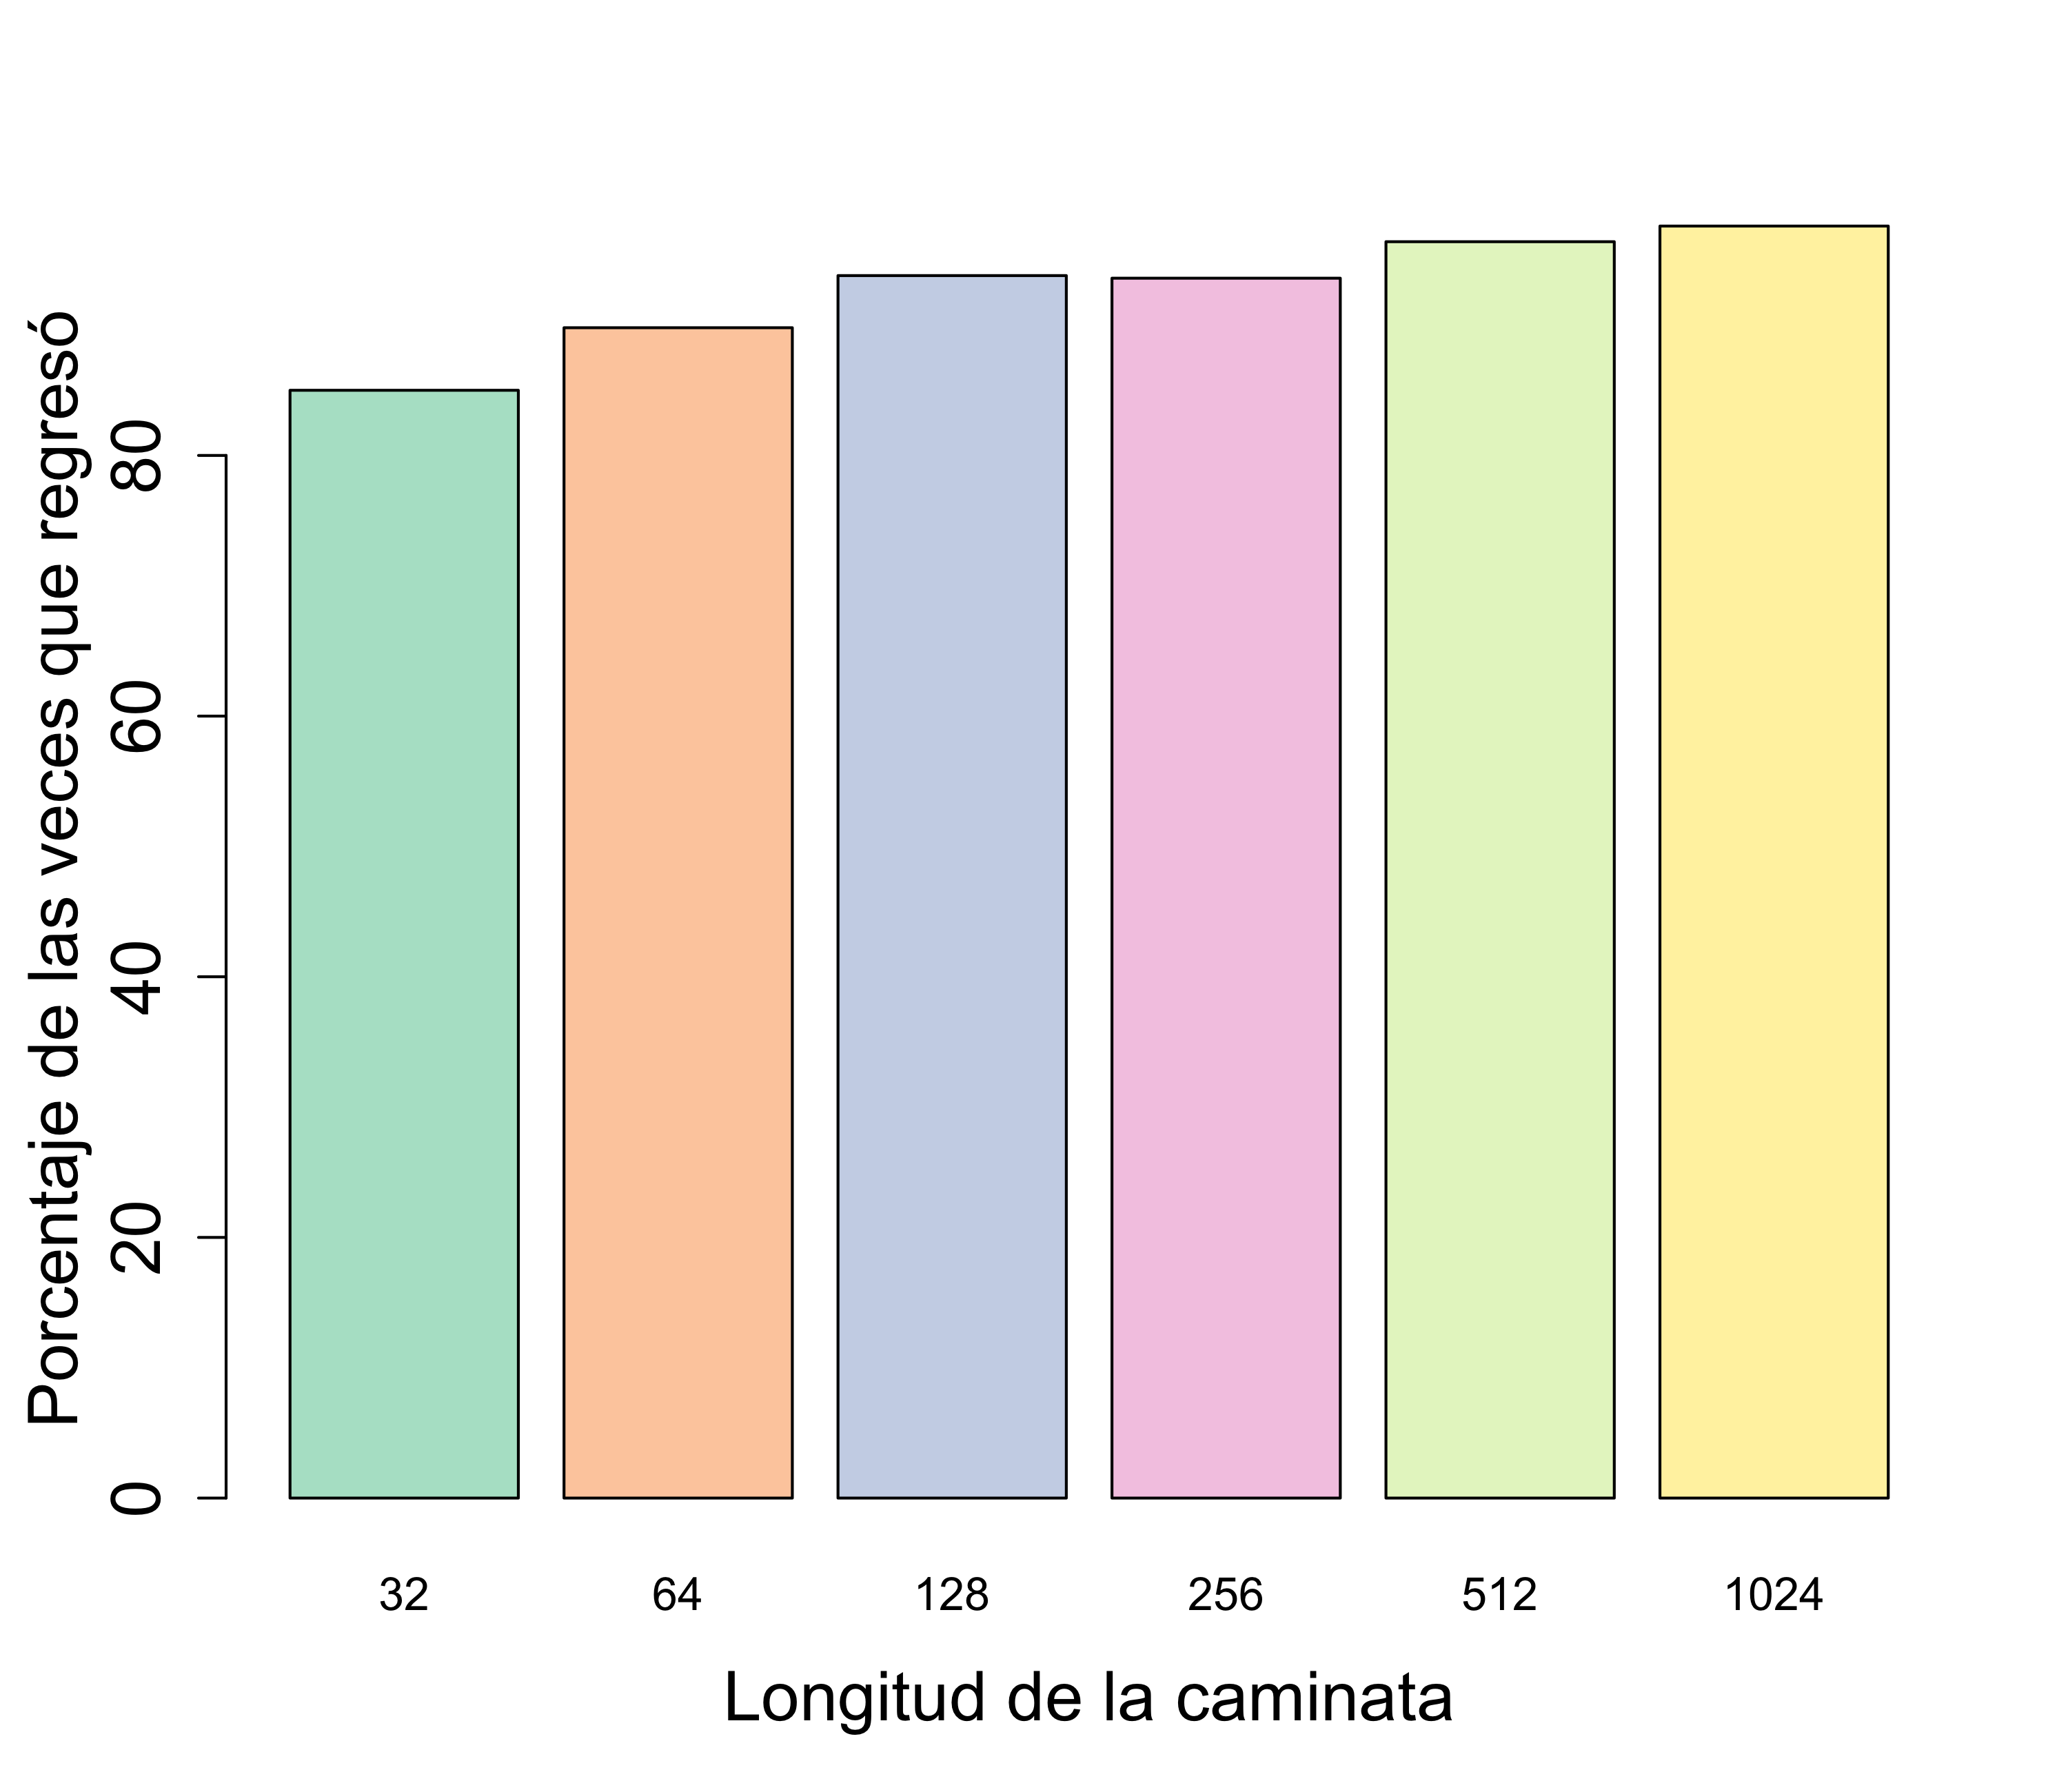
\includegraphics[width=\linewidth]{Dimension1-prob.png}
 		 		\label{dim1}
 	\end{subfigure}
 	\begin{subfigure}[b]{0.3\linewidth}
 		\caption{Dimensión 2.}
 		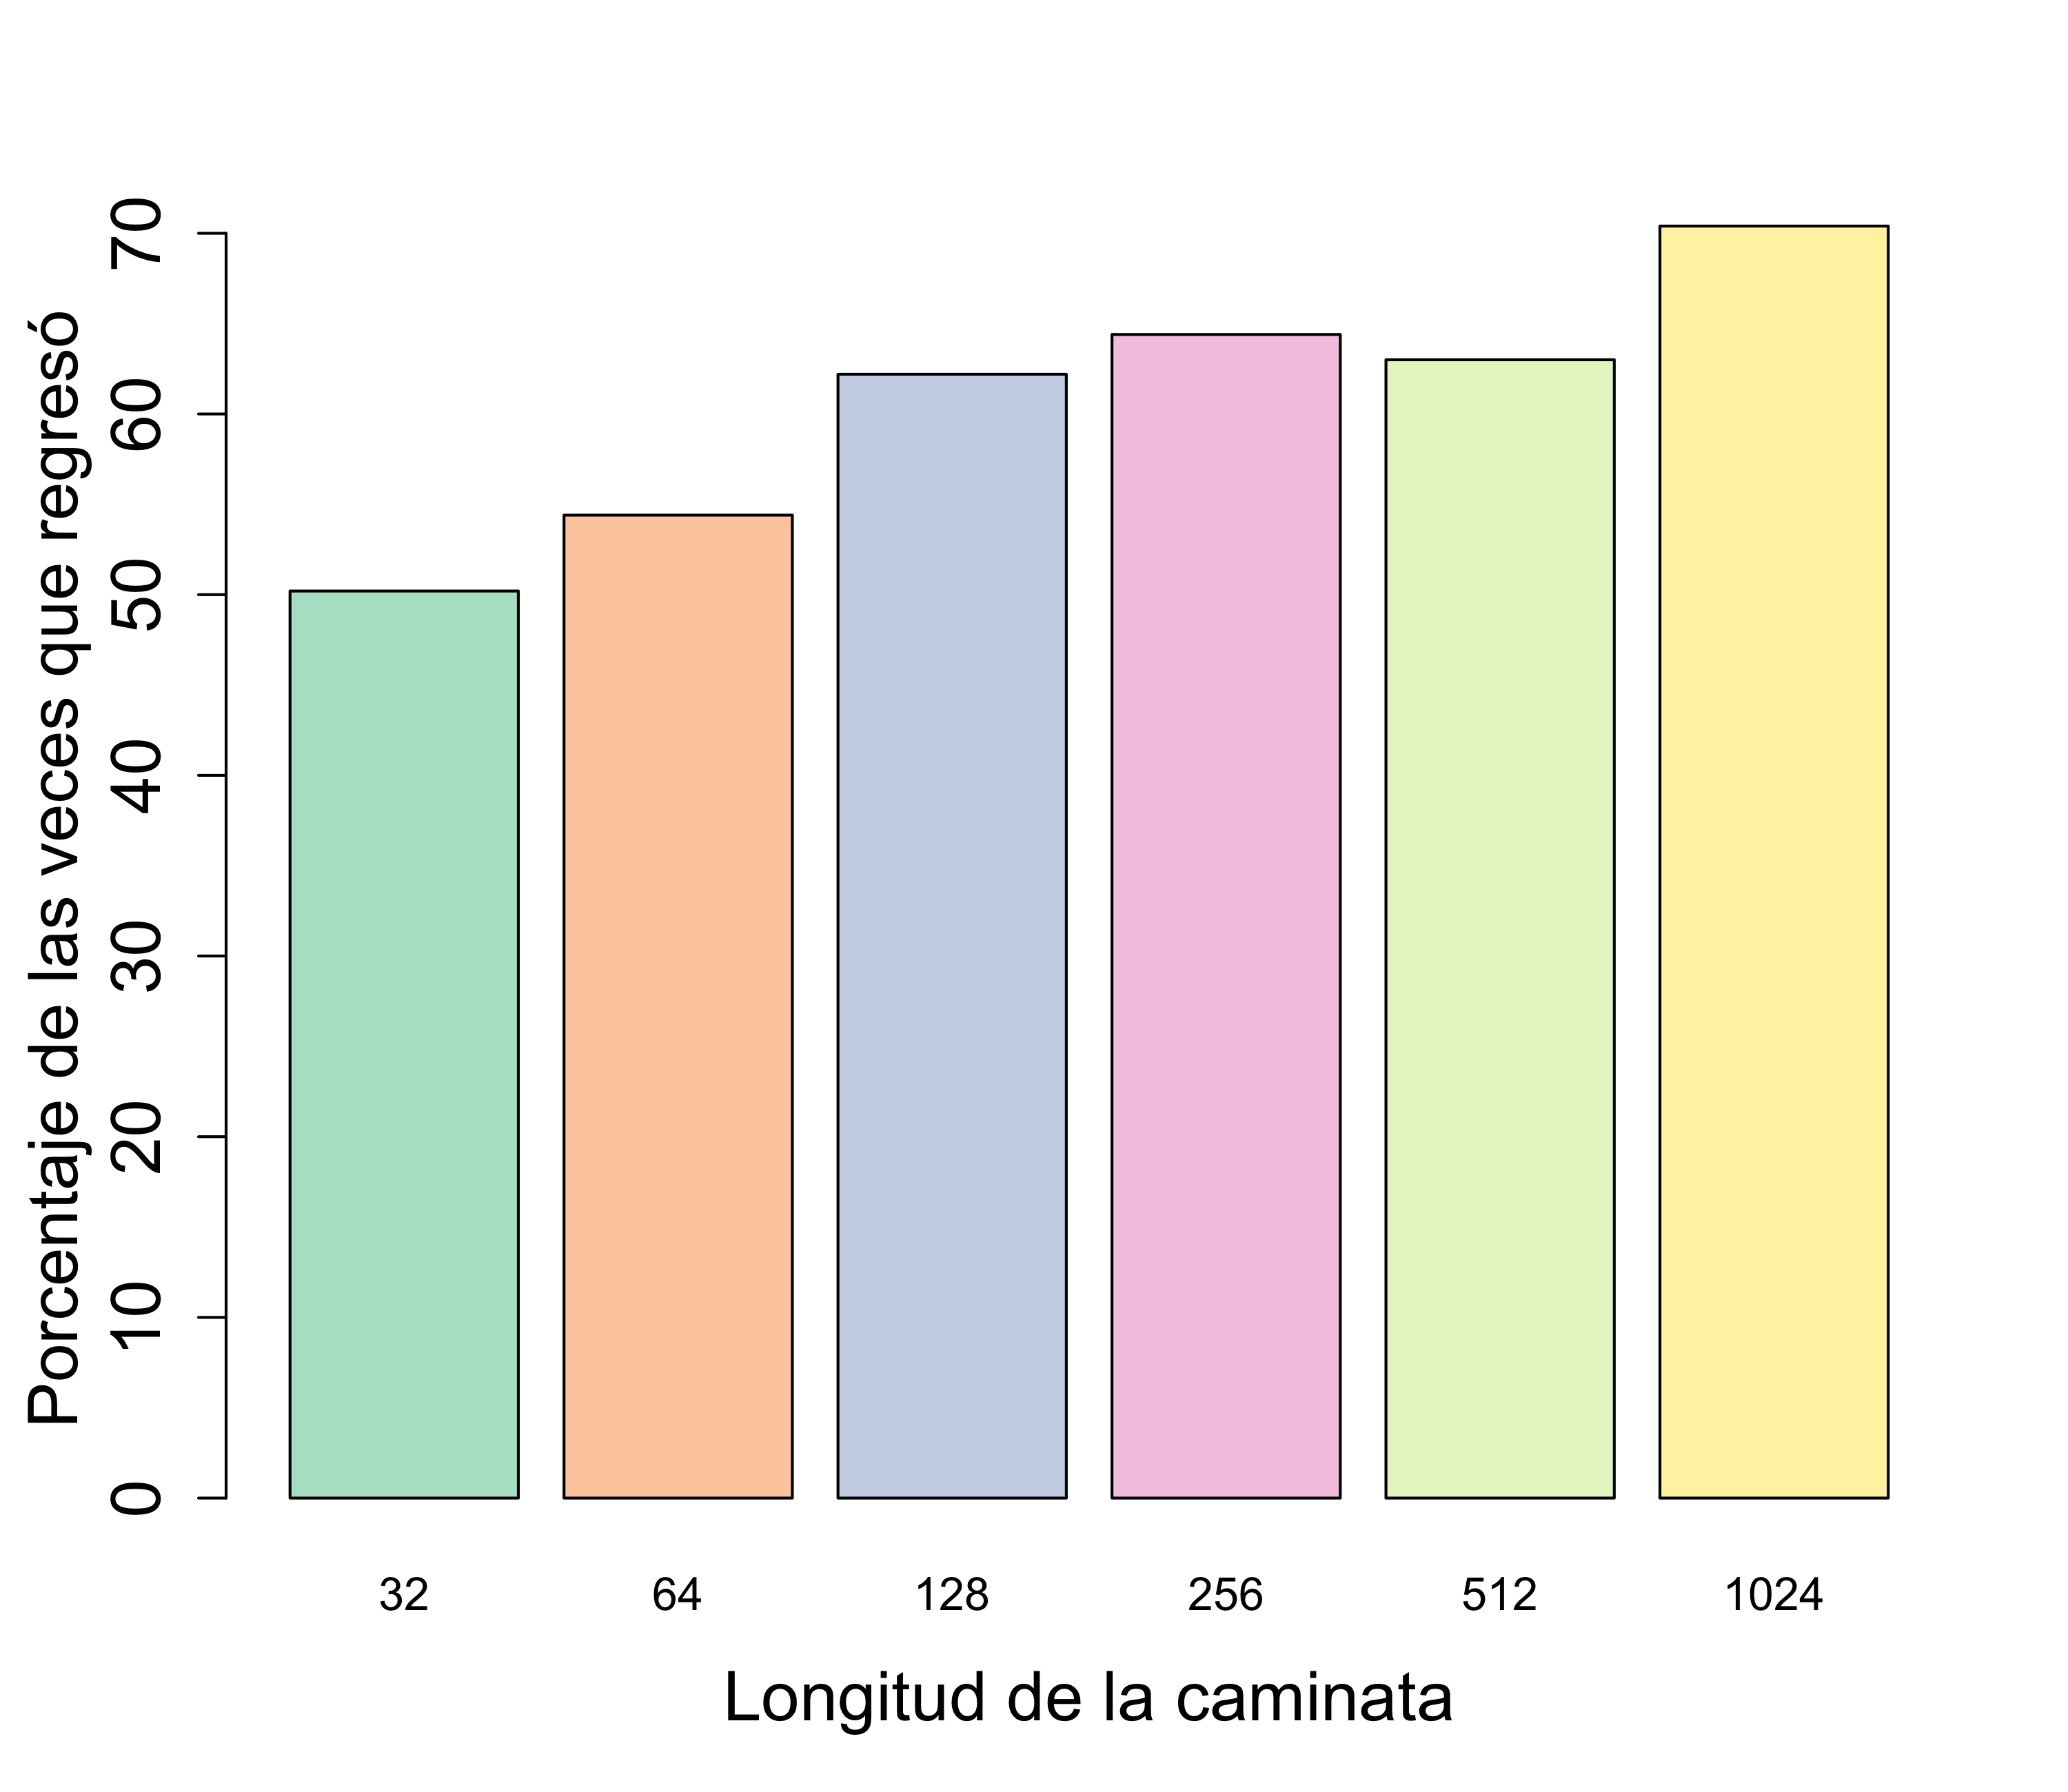
\includegraphics[width=\linewidth]{Dimension2-prob.png}
 		\label{dim2}
 	\end{subfigure}
 	\begin{subfigure}[b]{0.3\linewidth}
 		\caption{Dimensión 3.}
 		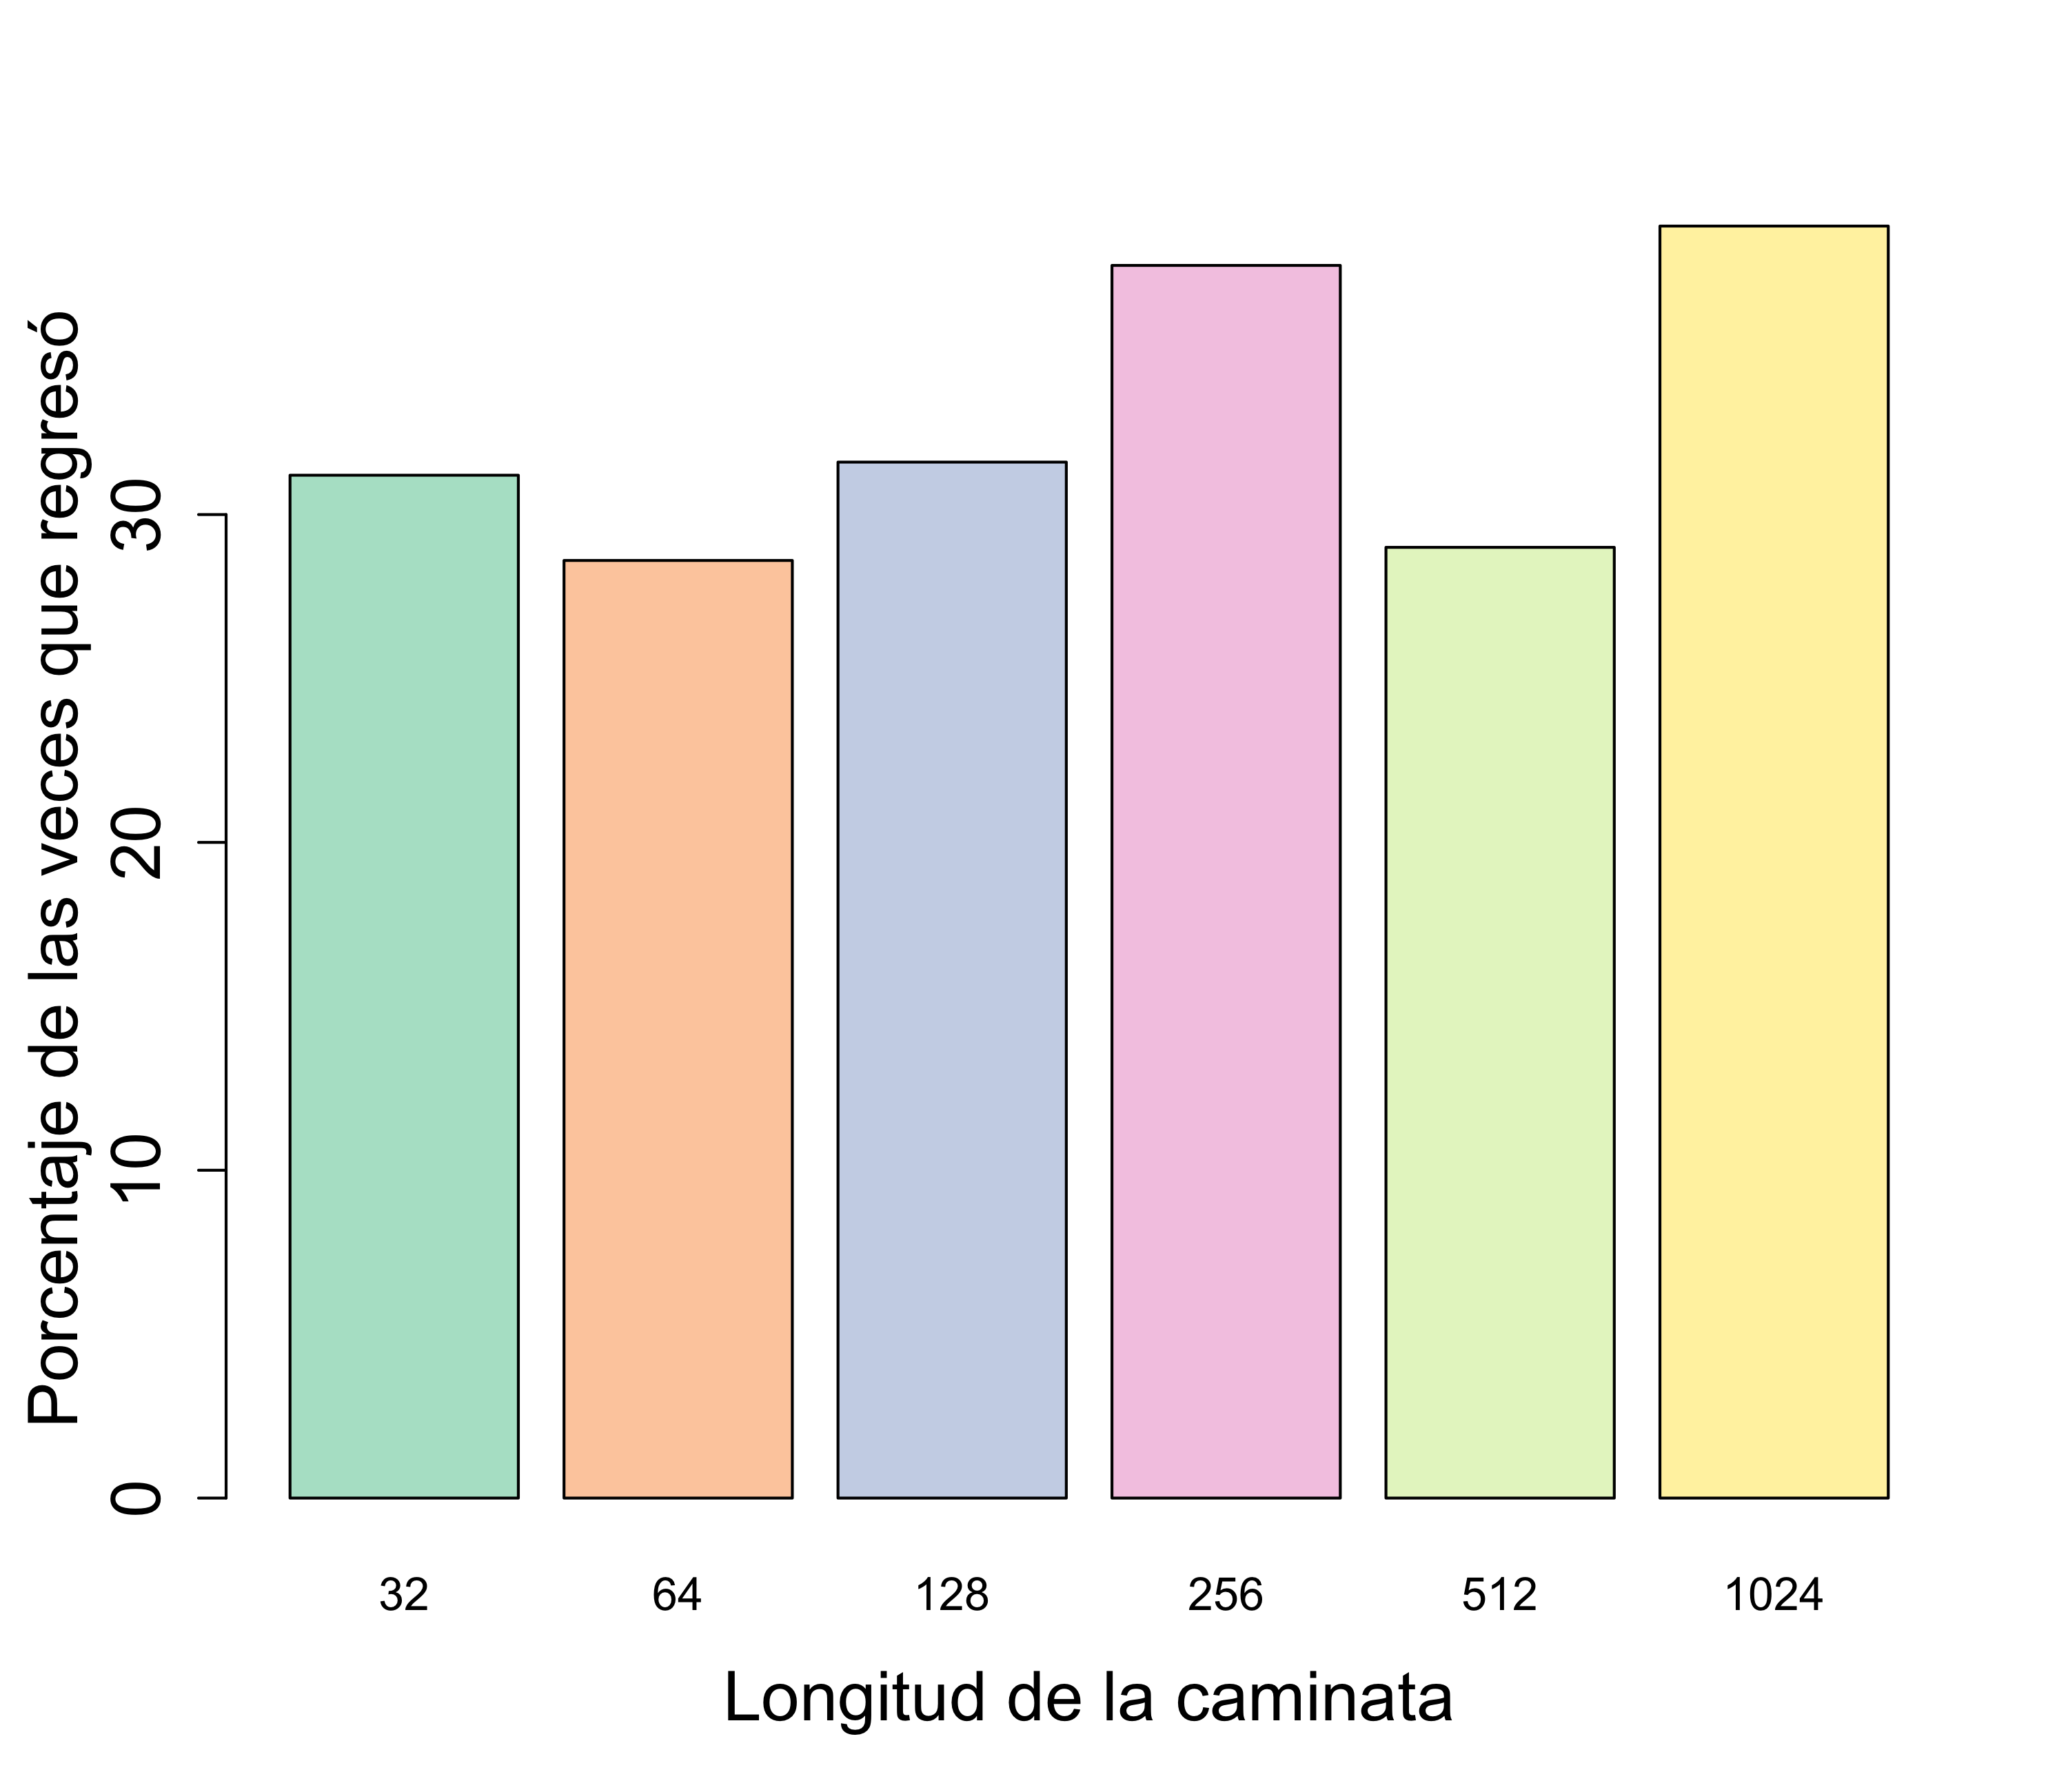
\includegraphics[width=\linewidth]{Dimension3-prob.png}
 		\label{dim3}
 	\end{subfigure}
	\begin{subfigure}[b]{0.3\linewidth}
 		\caption{Dimensión 4.}
 		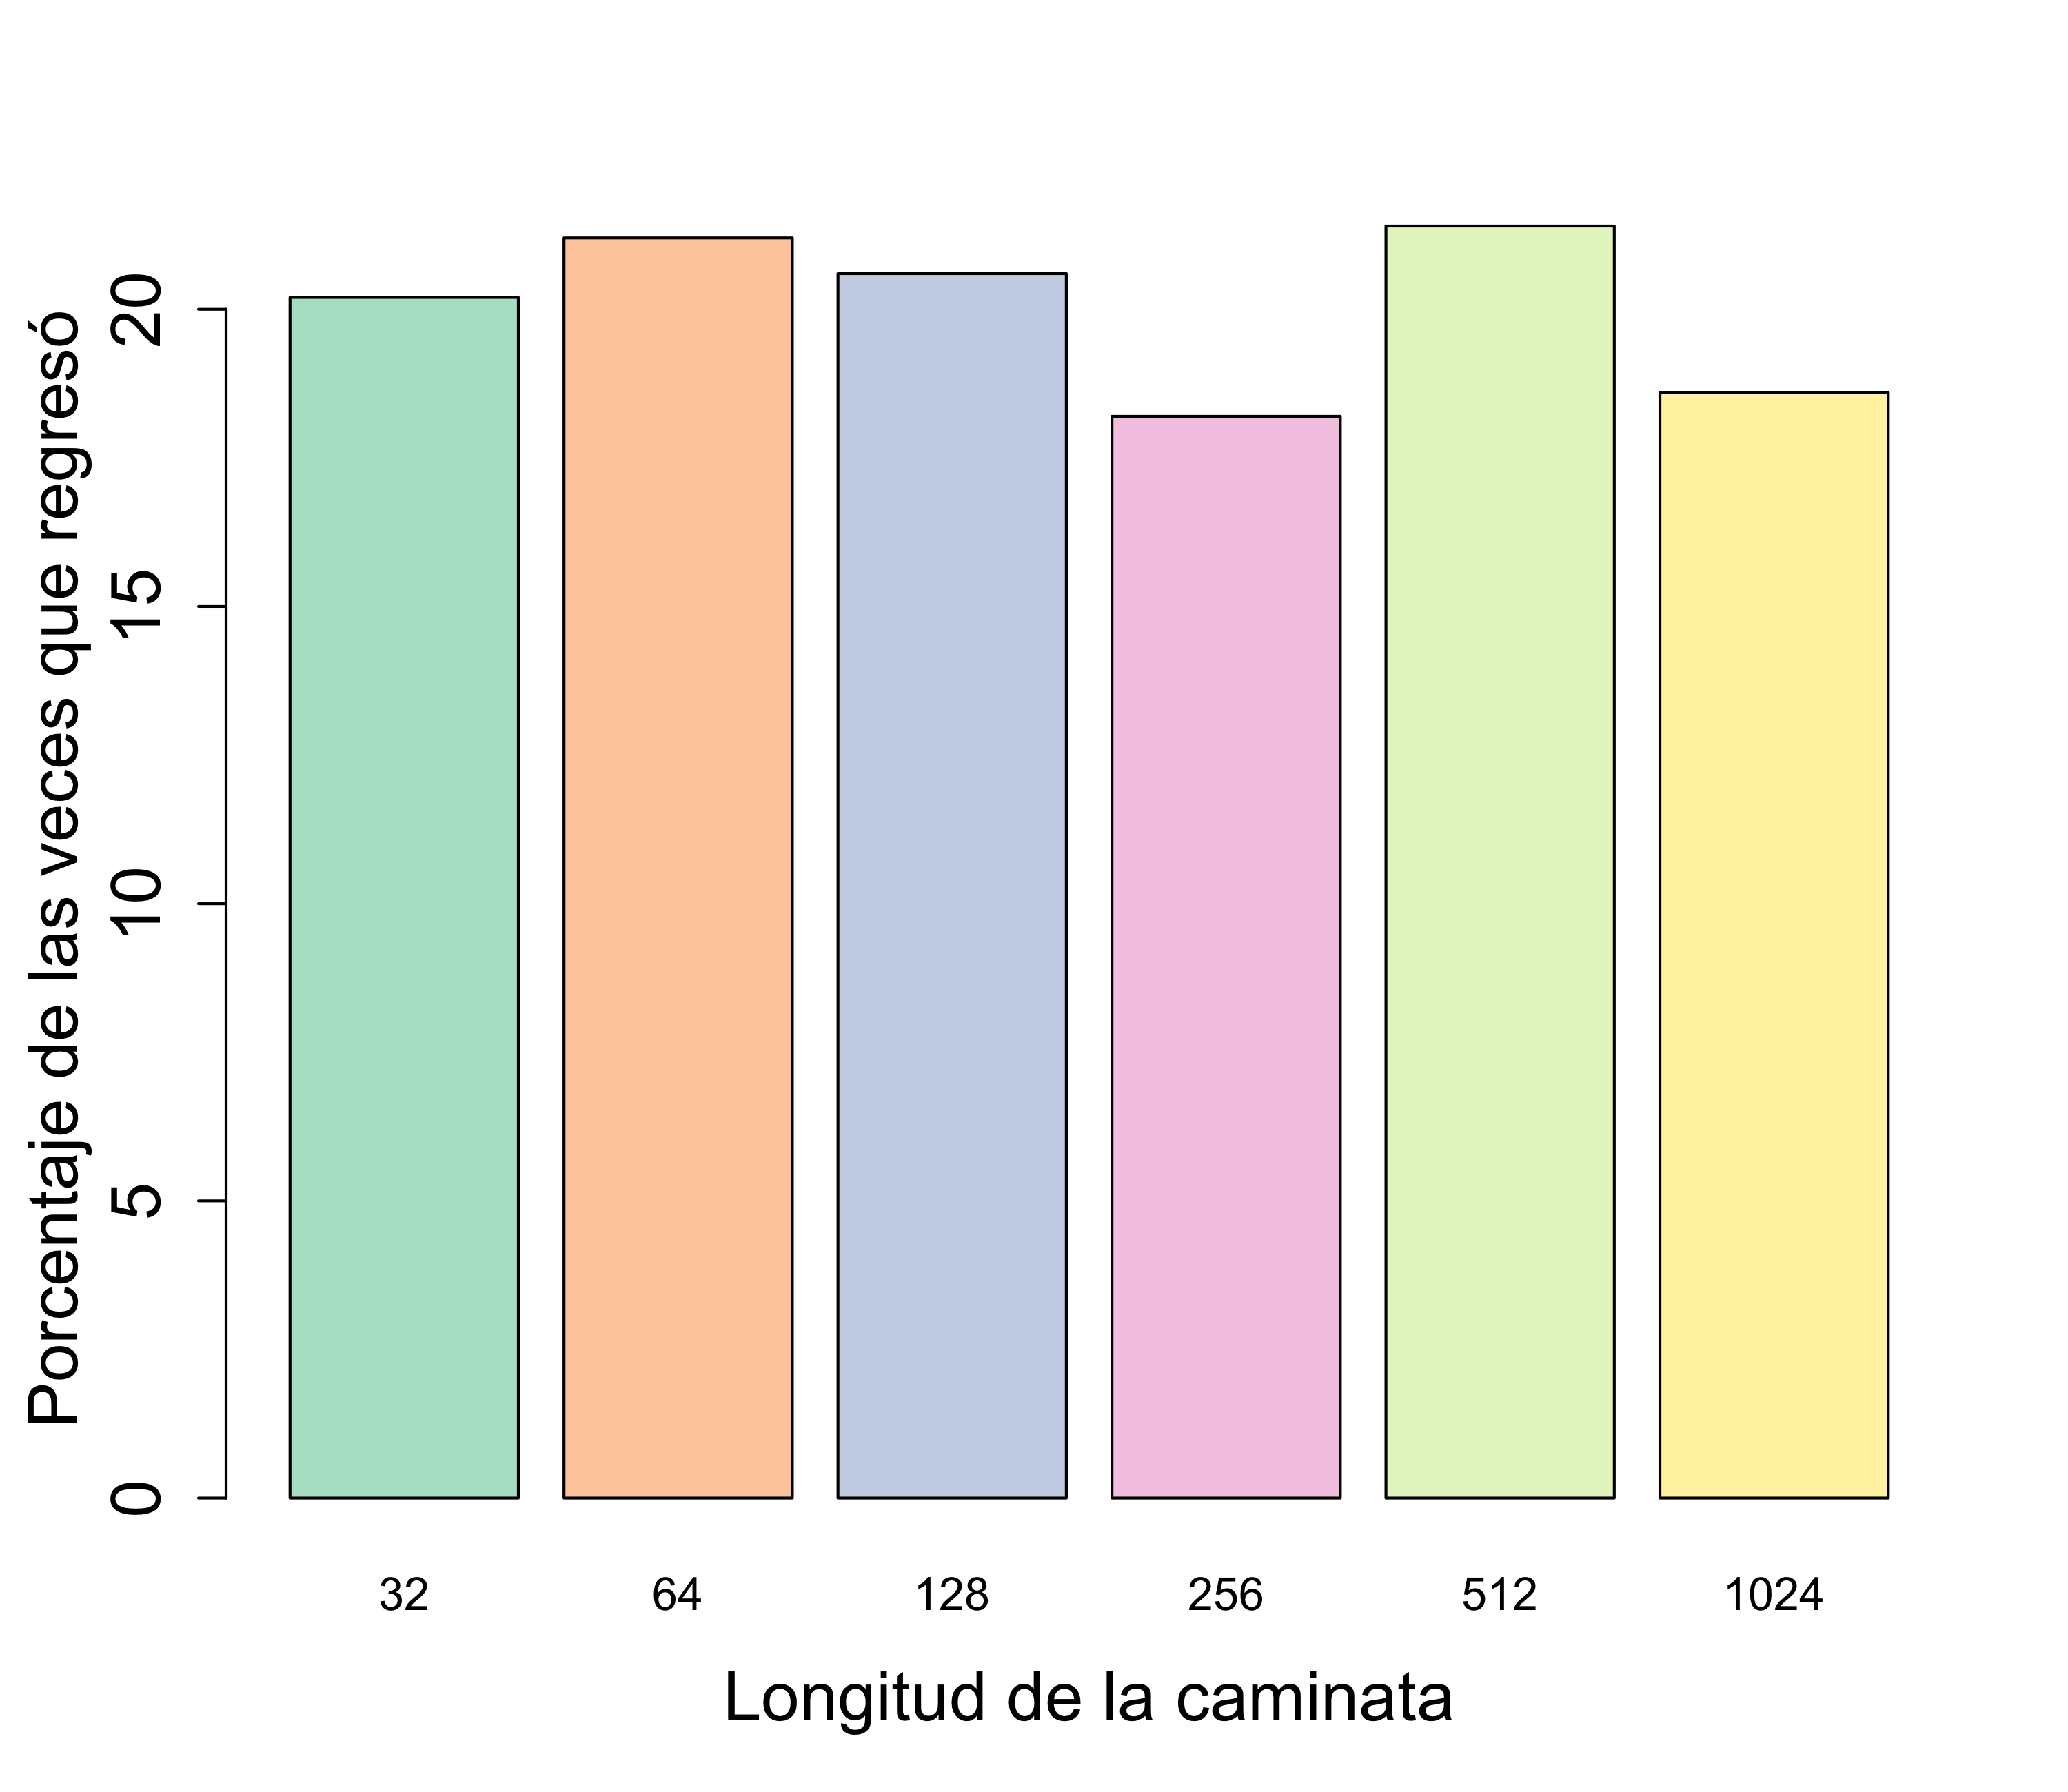
\includegraphics[width=\linewidth]{Dimension4-prob.png}
 		\label{dim4}
 	\end{subfigure}
 		\begin{subfigure}[b]{0.3\linewidth}
 		\caption{Dimensión 5.}
 		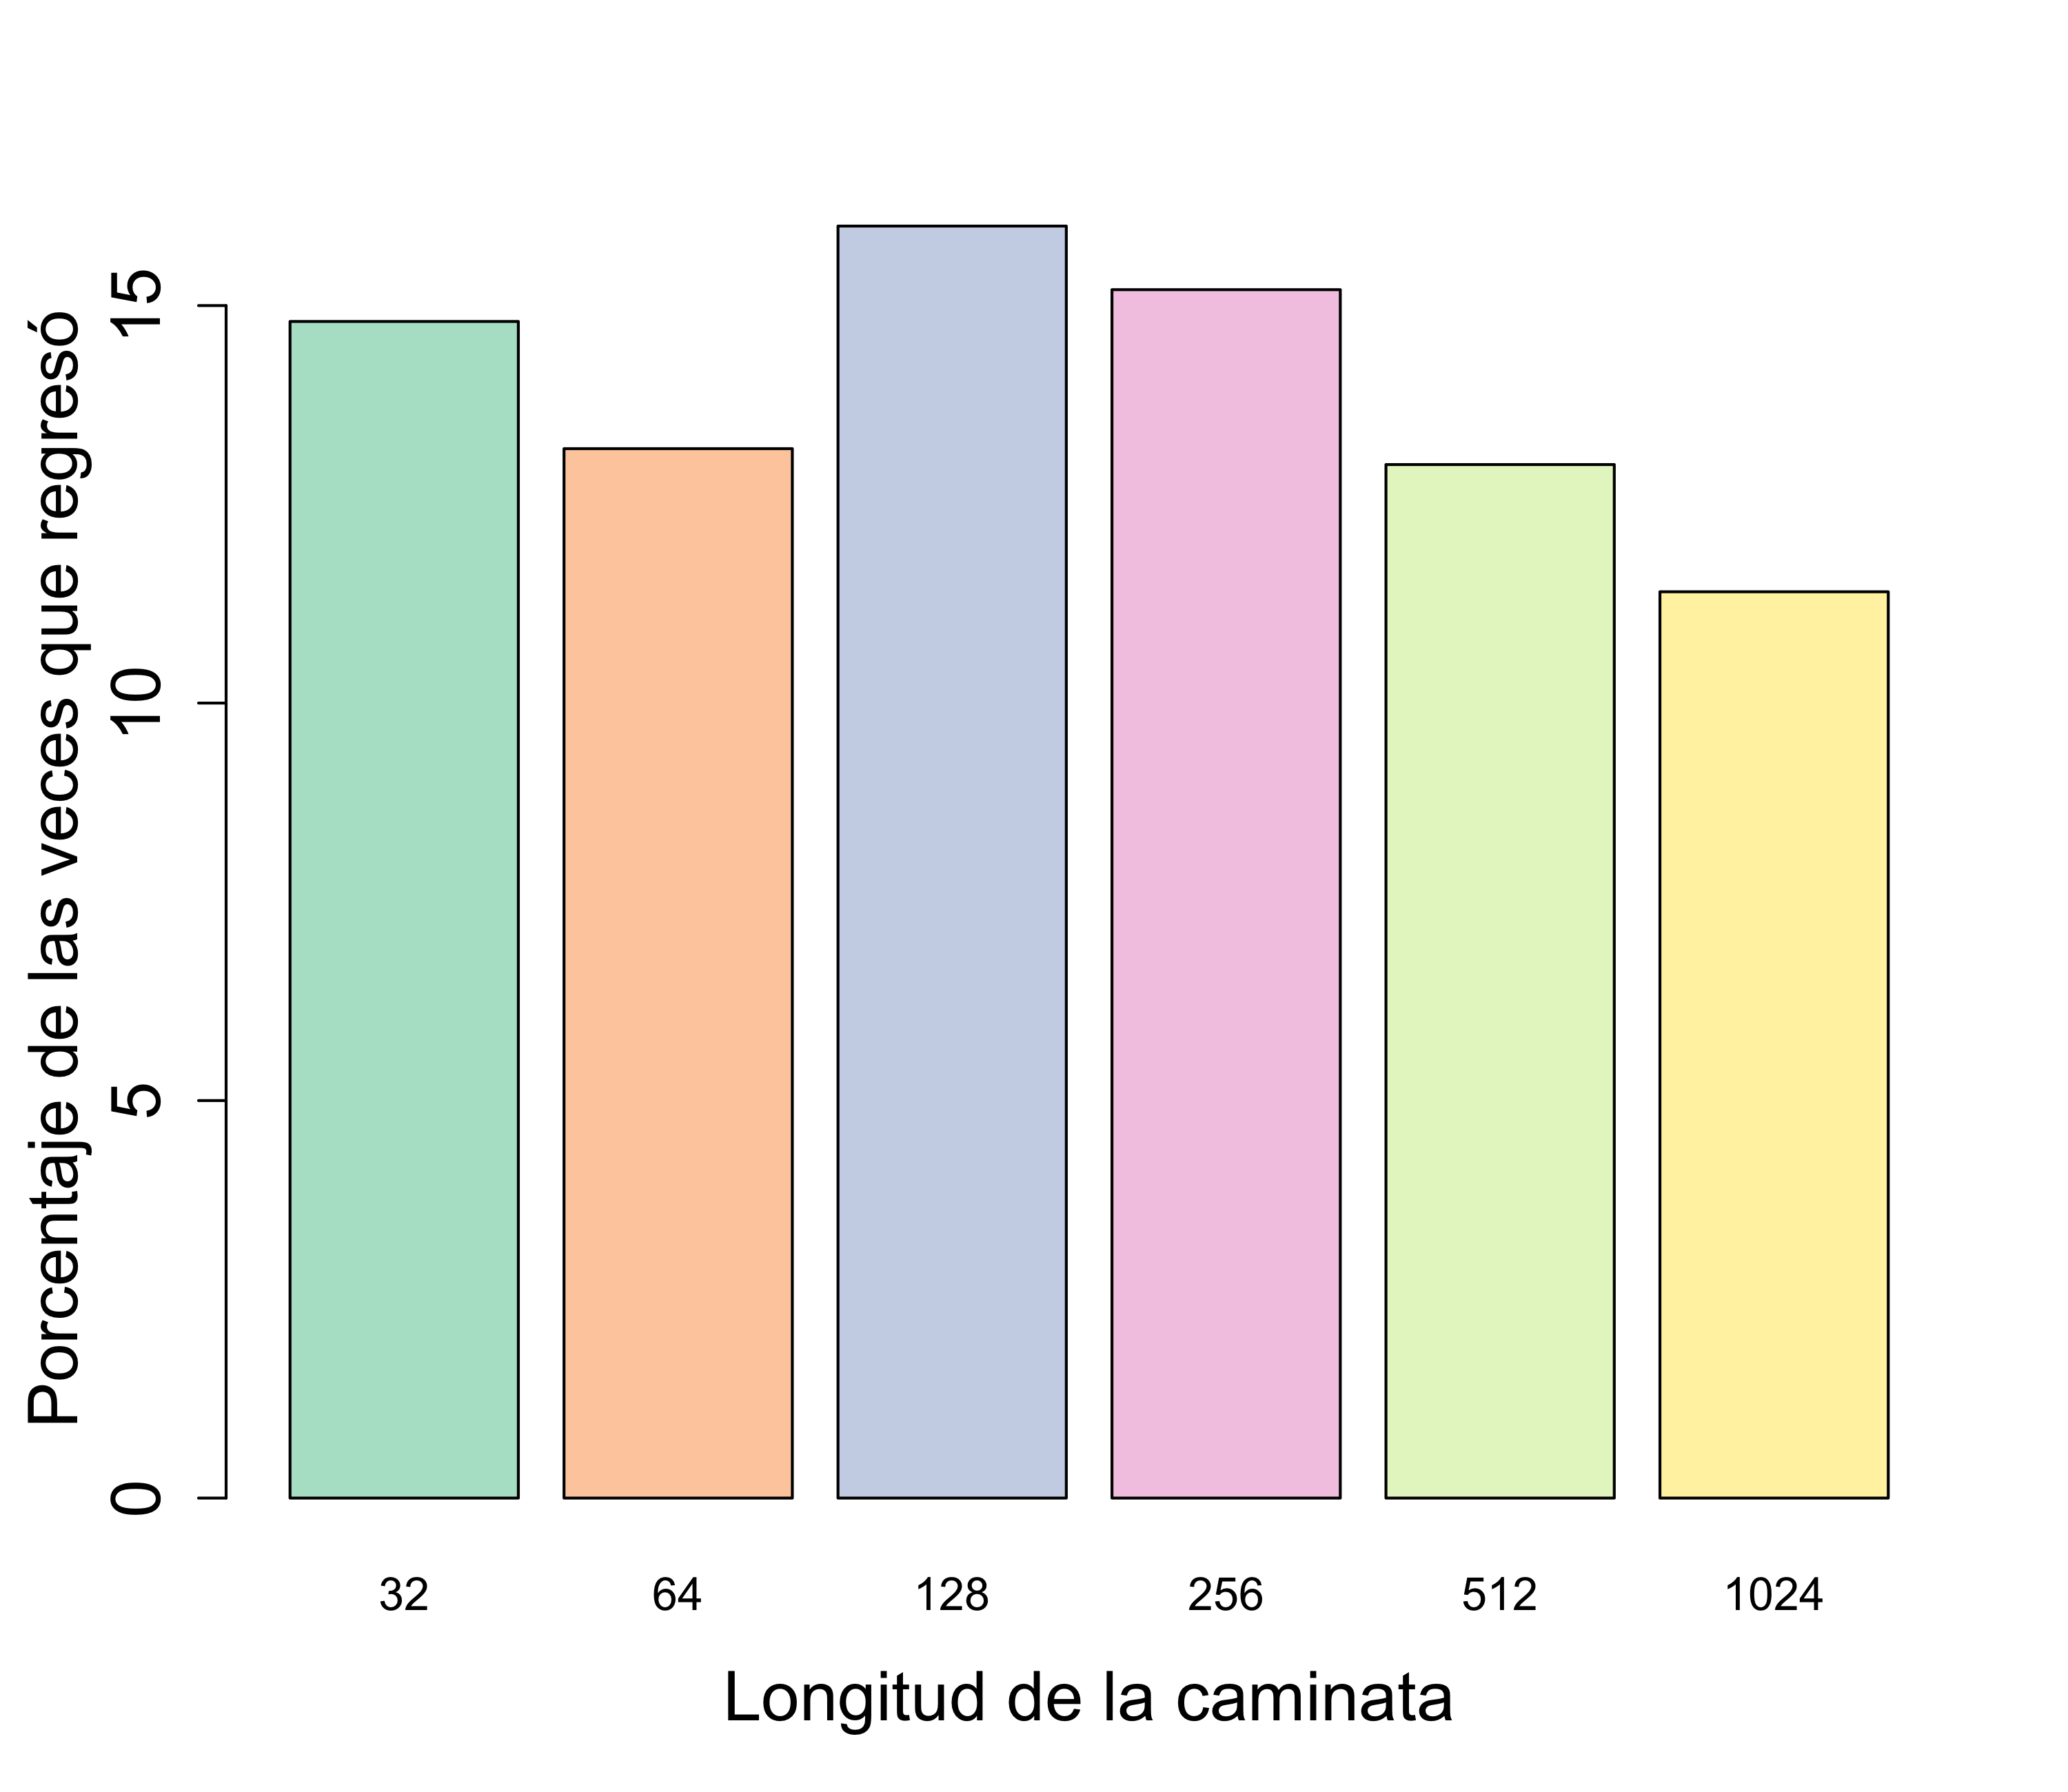
\includegraphics[width=\linewidth]{Dimension5-prob.png}
 		\label{dim5}
 	\end{subfigure}
 		\begin{subfigure}[b]{0.3\linewidth}
 		\caption{Dimensión 6.}
 		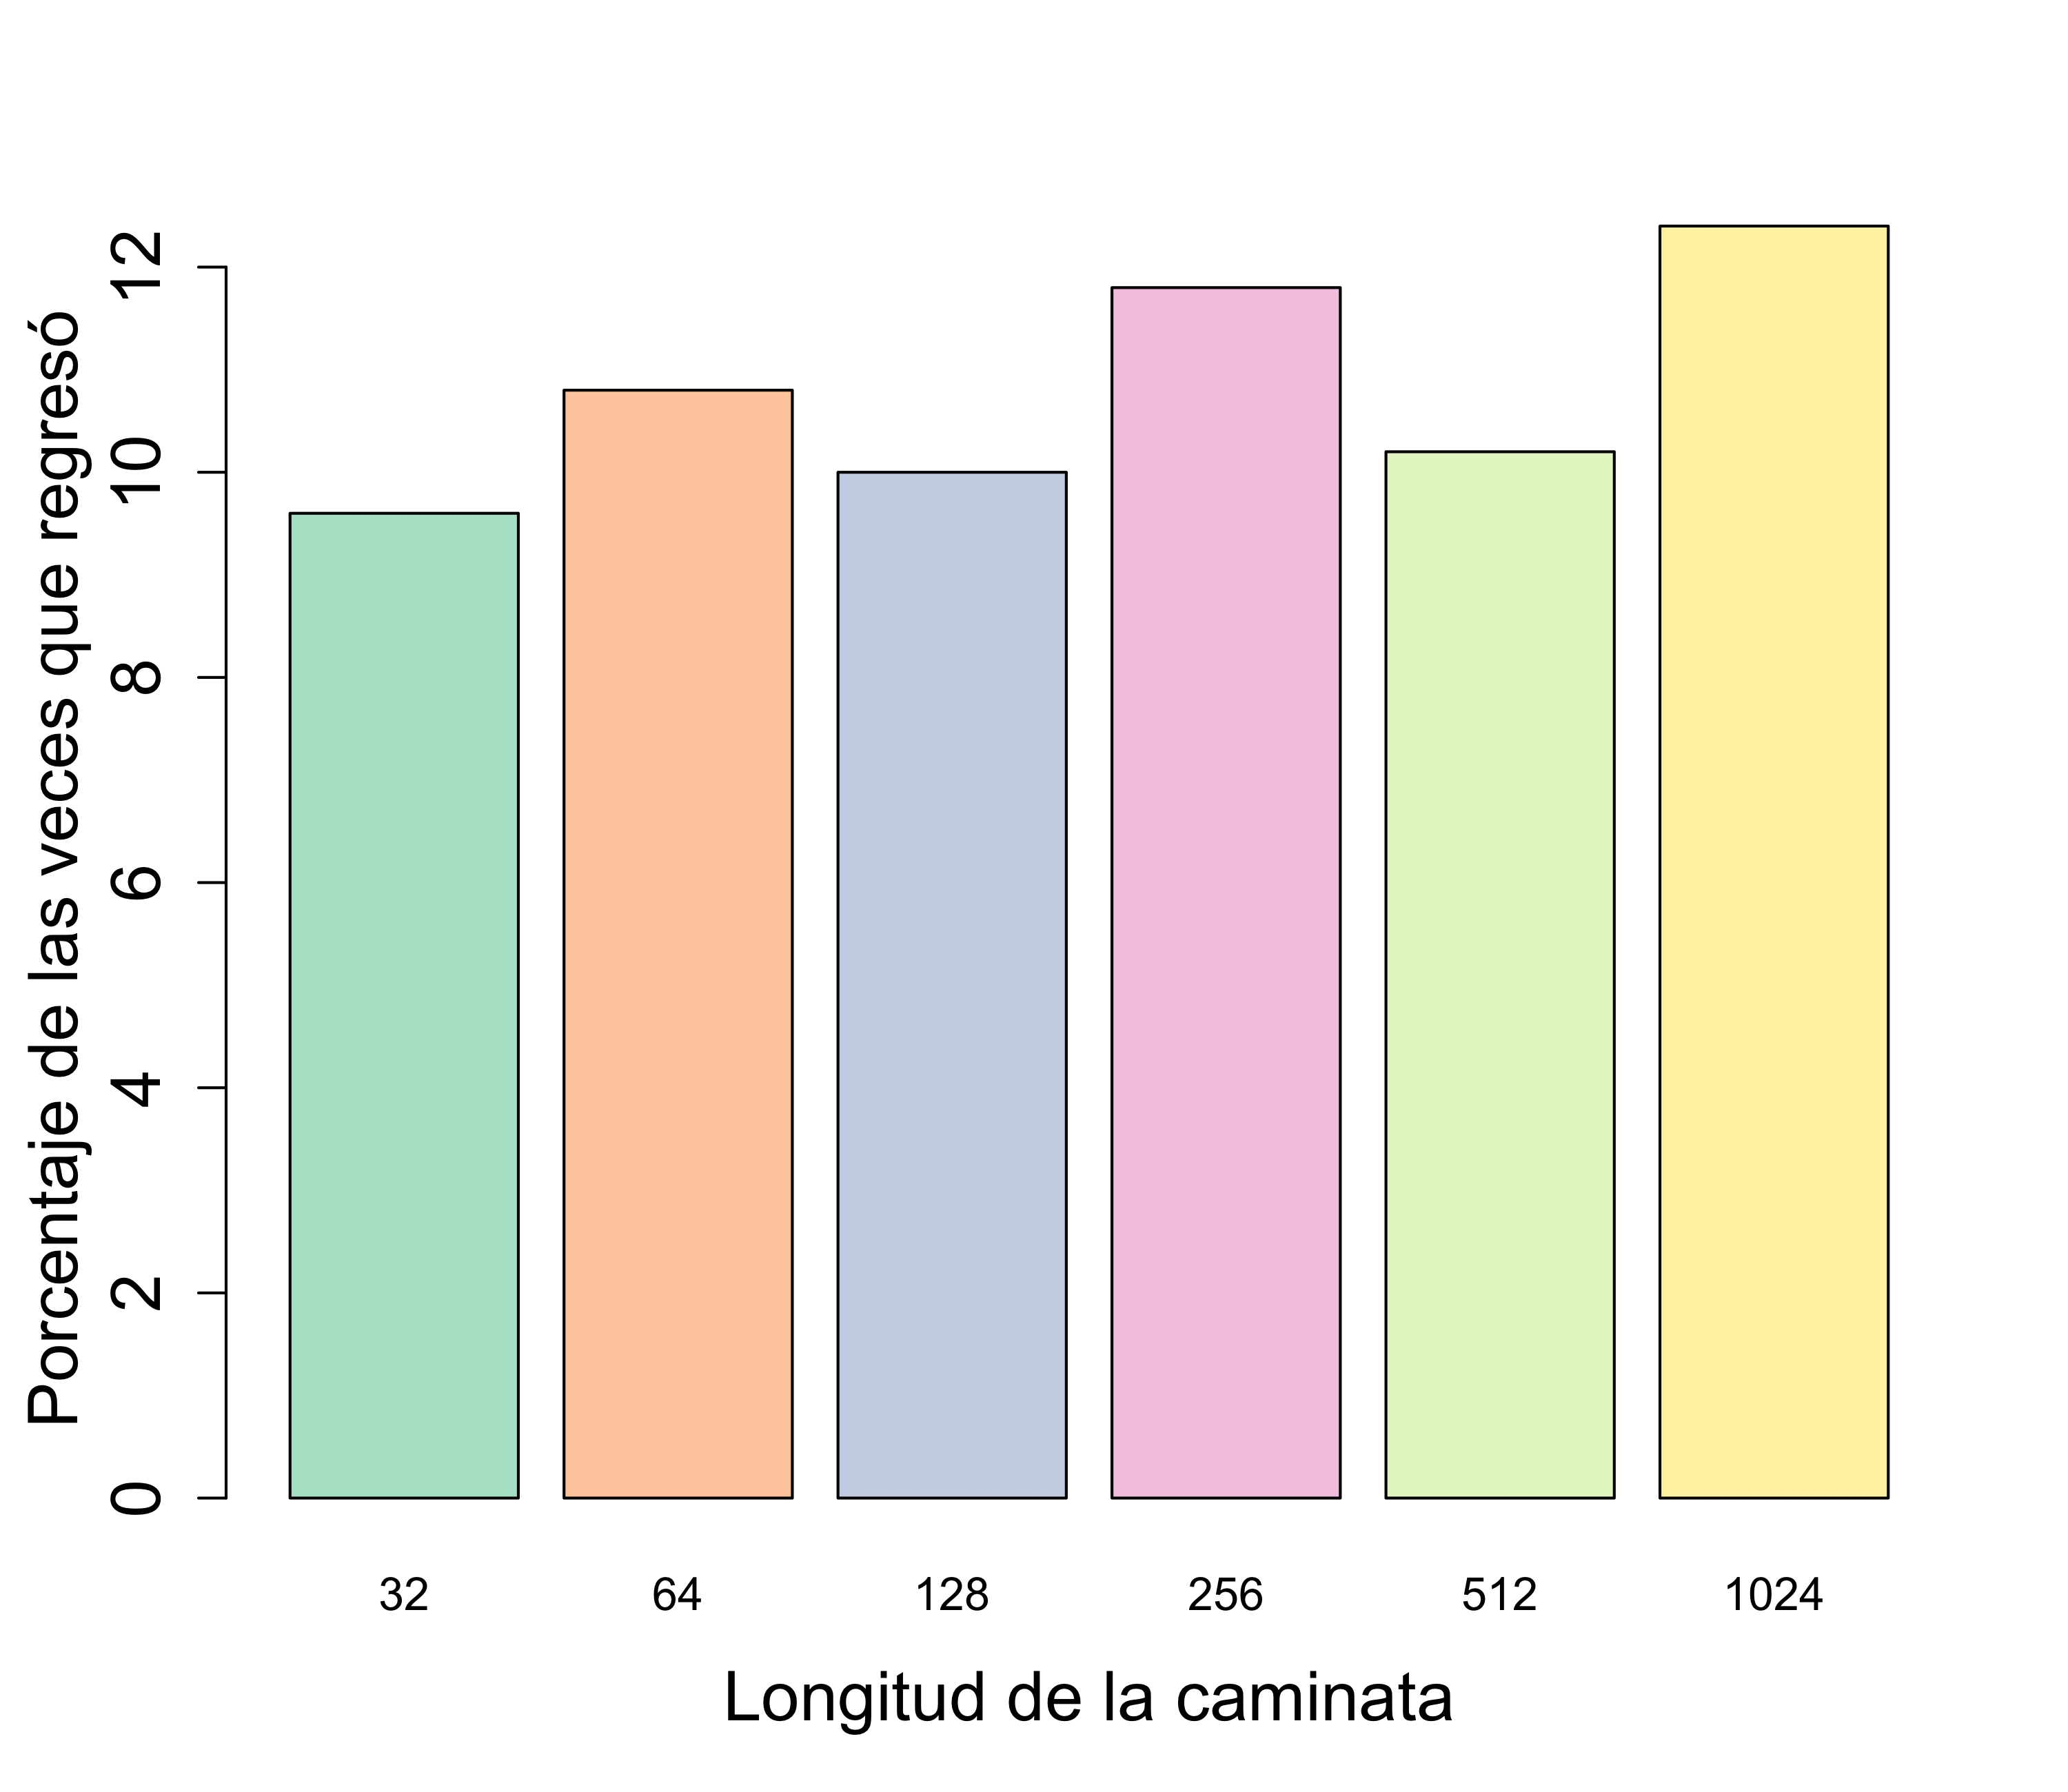
\includegraphics[width=\linewidth]{Dimension6-prob.png}
 		\label{dim6}
 	\end{subfigure}
 	\vspace{10cm}
 		\begin{subfigure}[b]{0.3\linewidth}
 		\caption{Dimensión 7.}
 		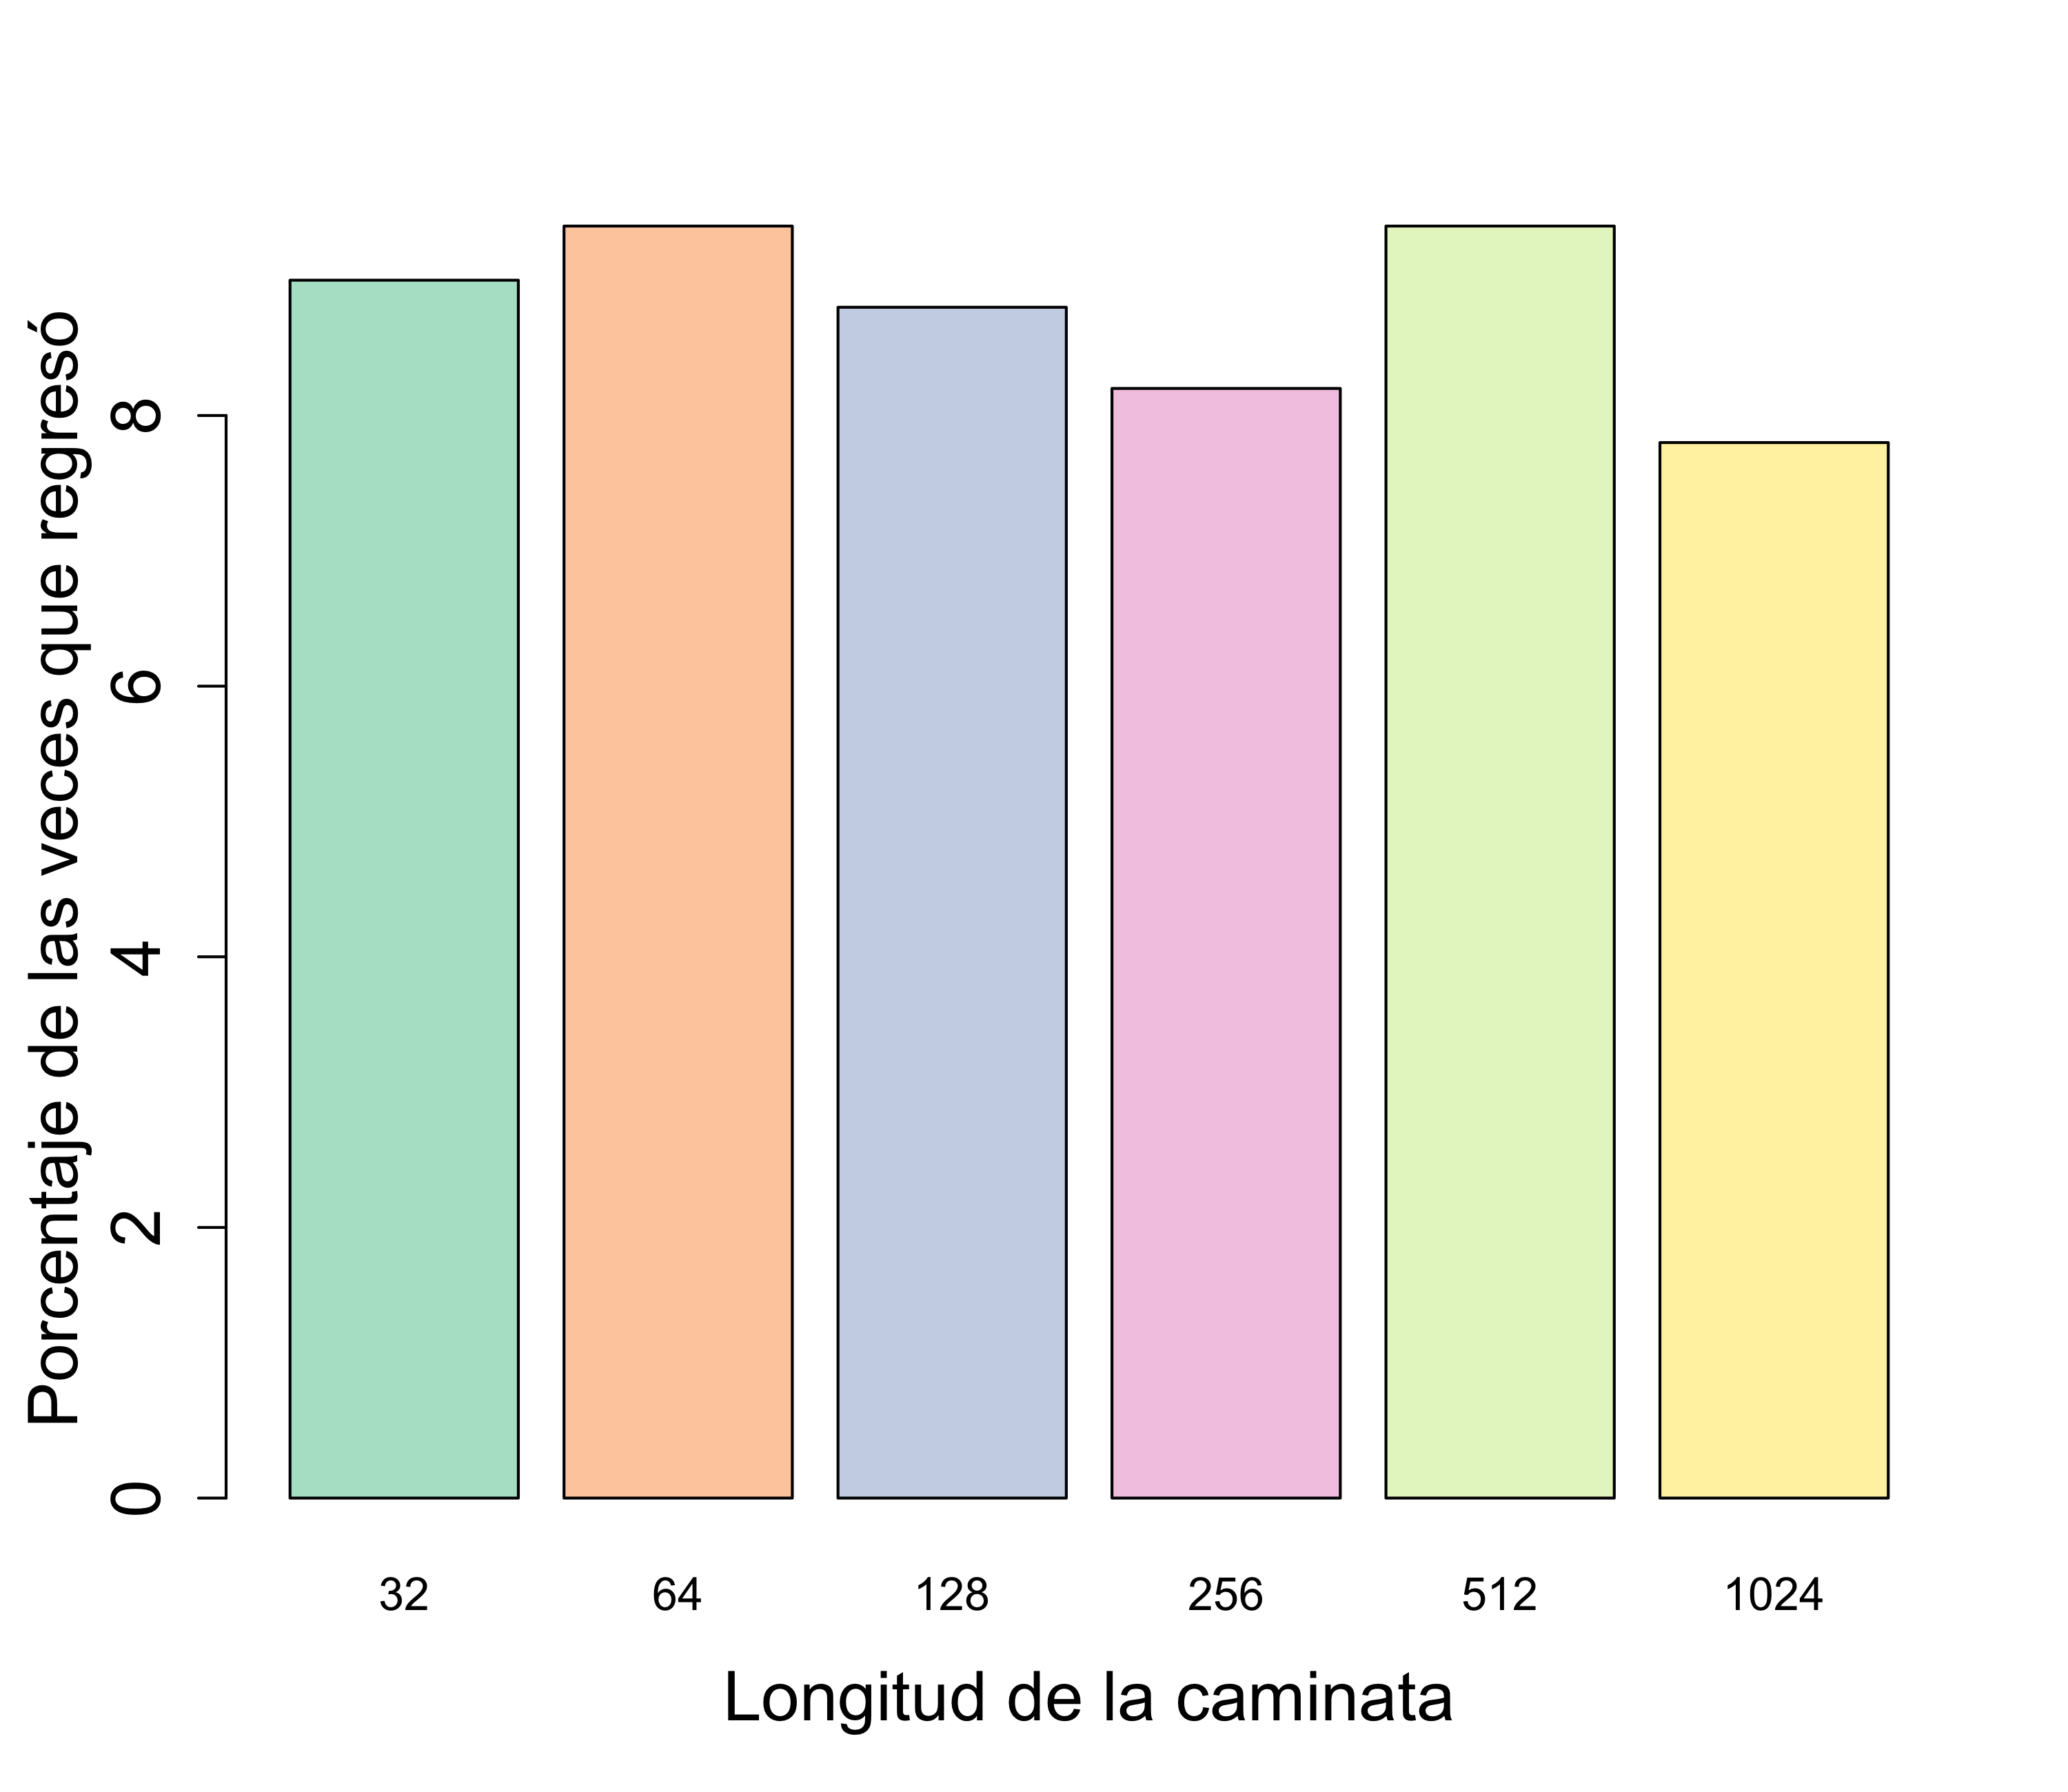
\includegraphics[width=\linewidth]{Dimension7-prob.png}
 		\label{dim7}
 	\end{subfigure}
 		\begin{subfigure}[b]{0.3\linewidth}
 		\caption{Dimensión 8.}
 		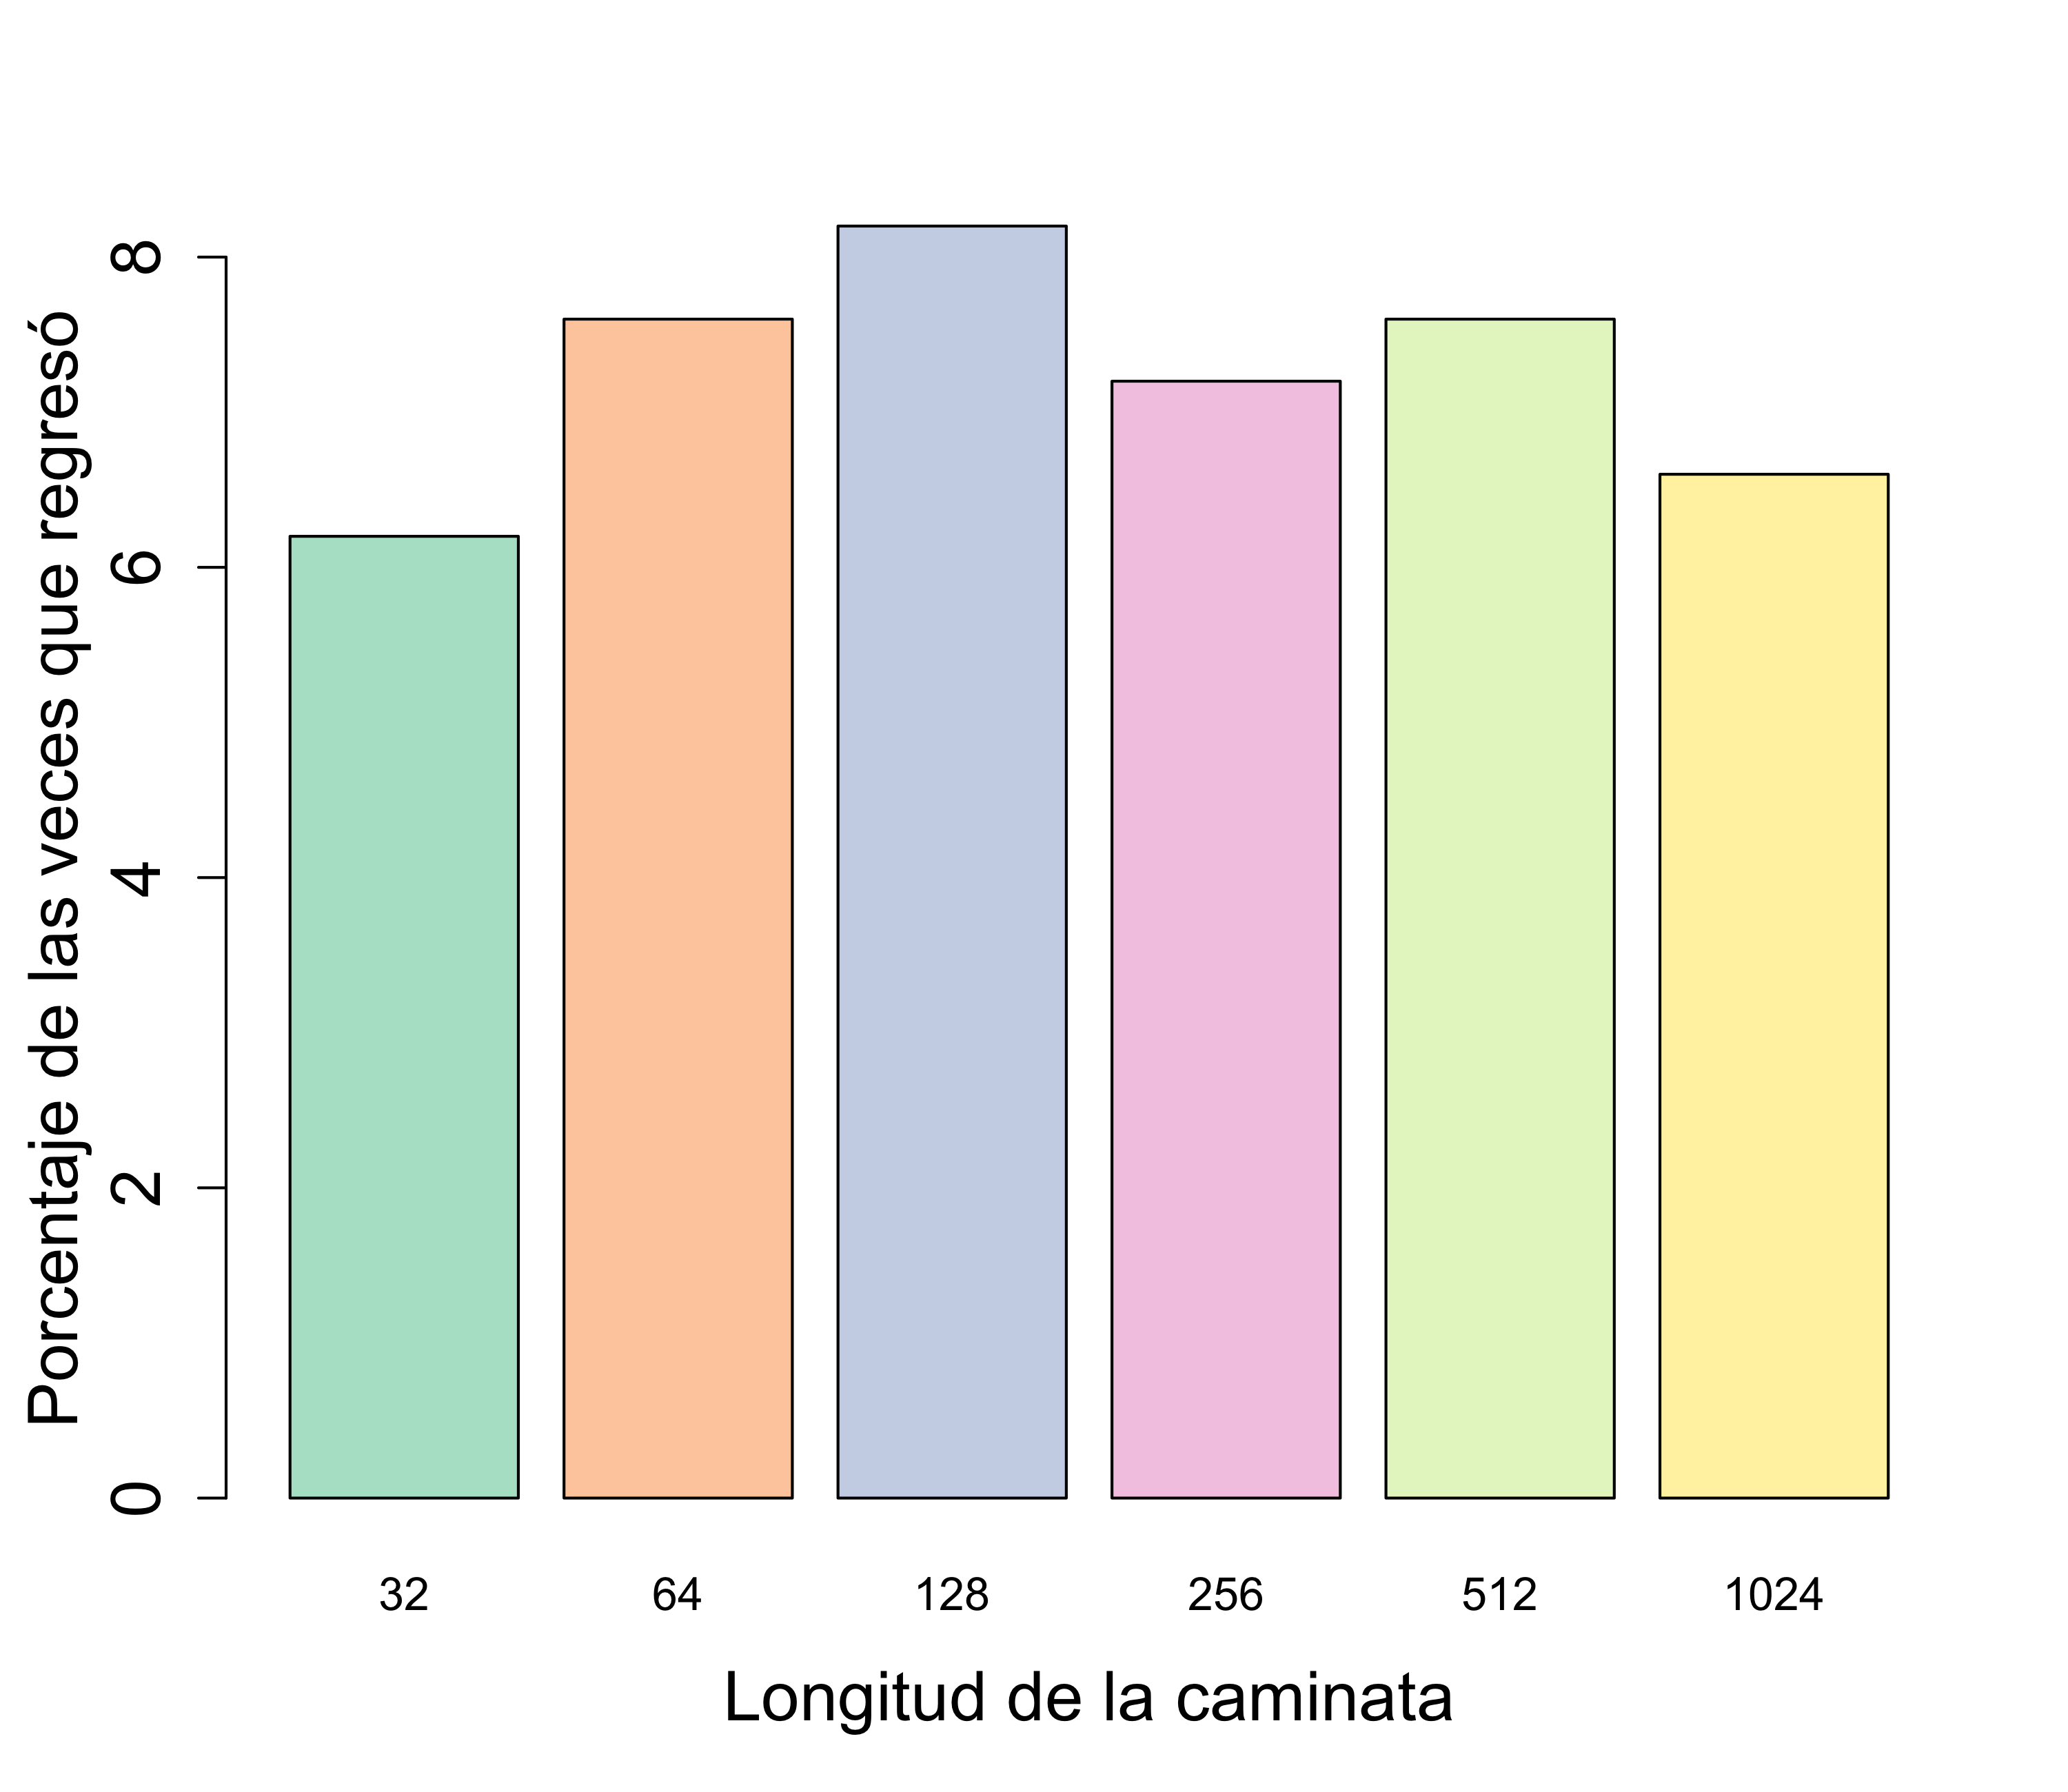
\includegraphics[width=\linewidth]{Dimension8-prob.png}
 		\label{dim8}
 	\end{subfigure}
 	\label{porcentajes}
 \end{figure}
 
 \begin{figure}
 	\centering
 	\caption{Pasos de regreso al origen en escala logarítmica.} 
 	\begin{subfigure}[b]{0.45\linewidth}
 		\caption{Caminata de 32 pasos.}
 		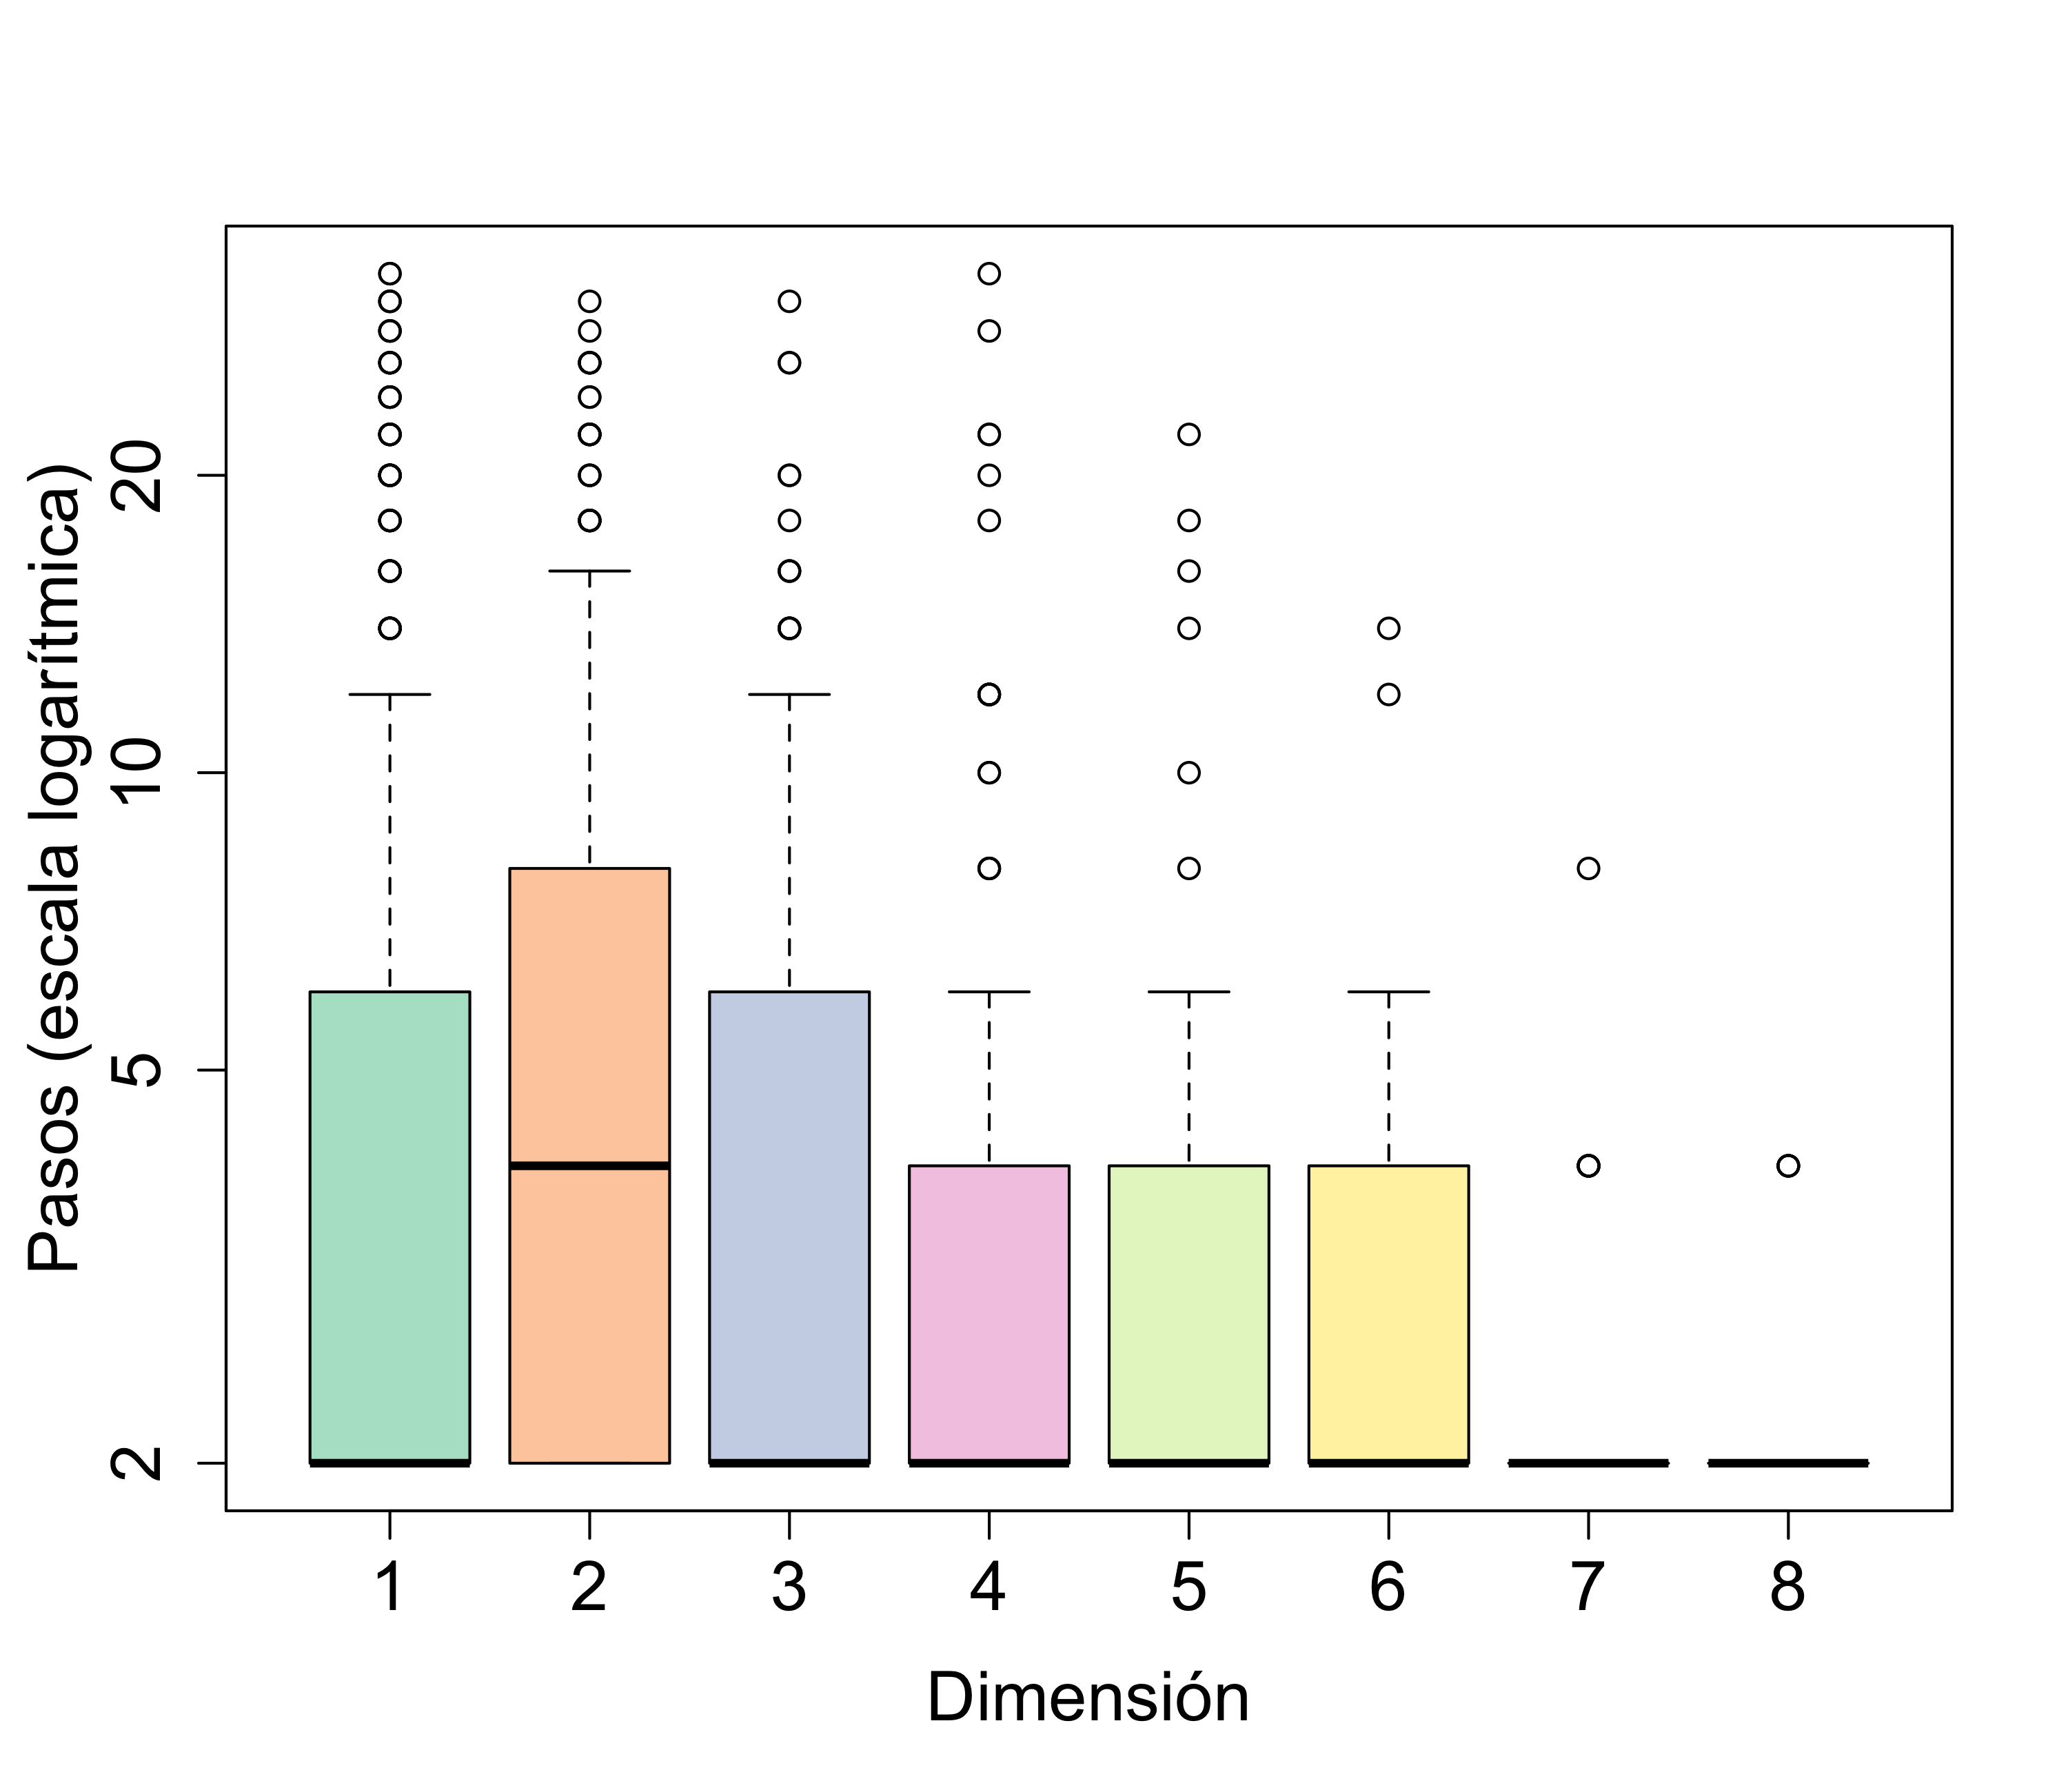
\includegraphics[width=\linewidth]{Largo32-pasos.png}
 		\label{32pasos}
 	\end{subfigure}
 	\begin{subfigure}[b]{0.45\linewidth}
 		\caption{Caminata de 64 pasos.}
 		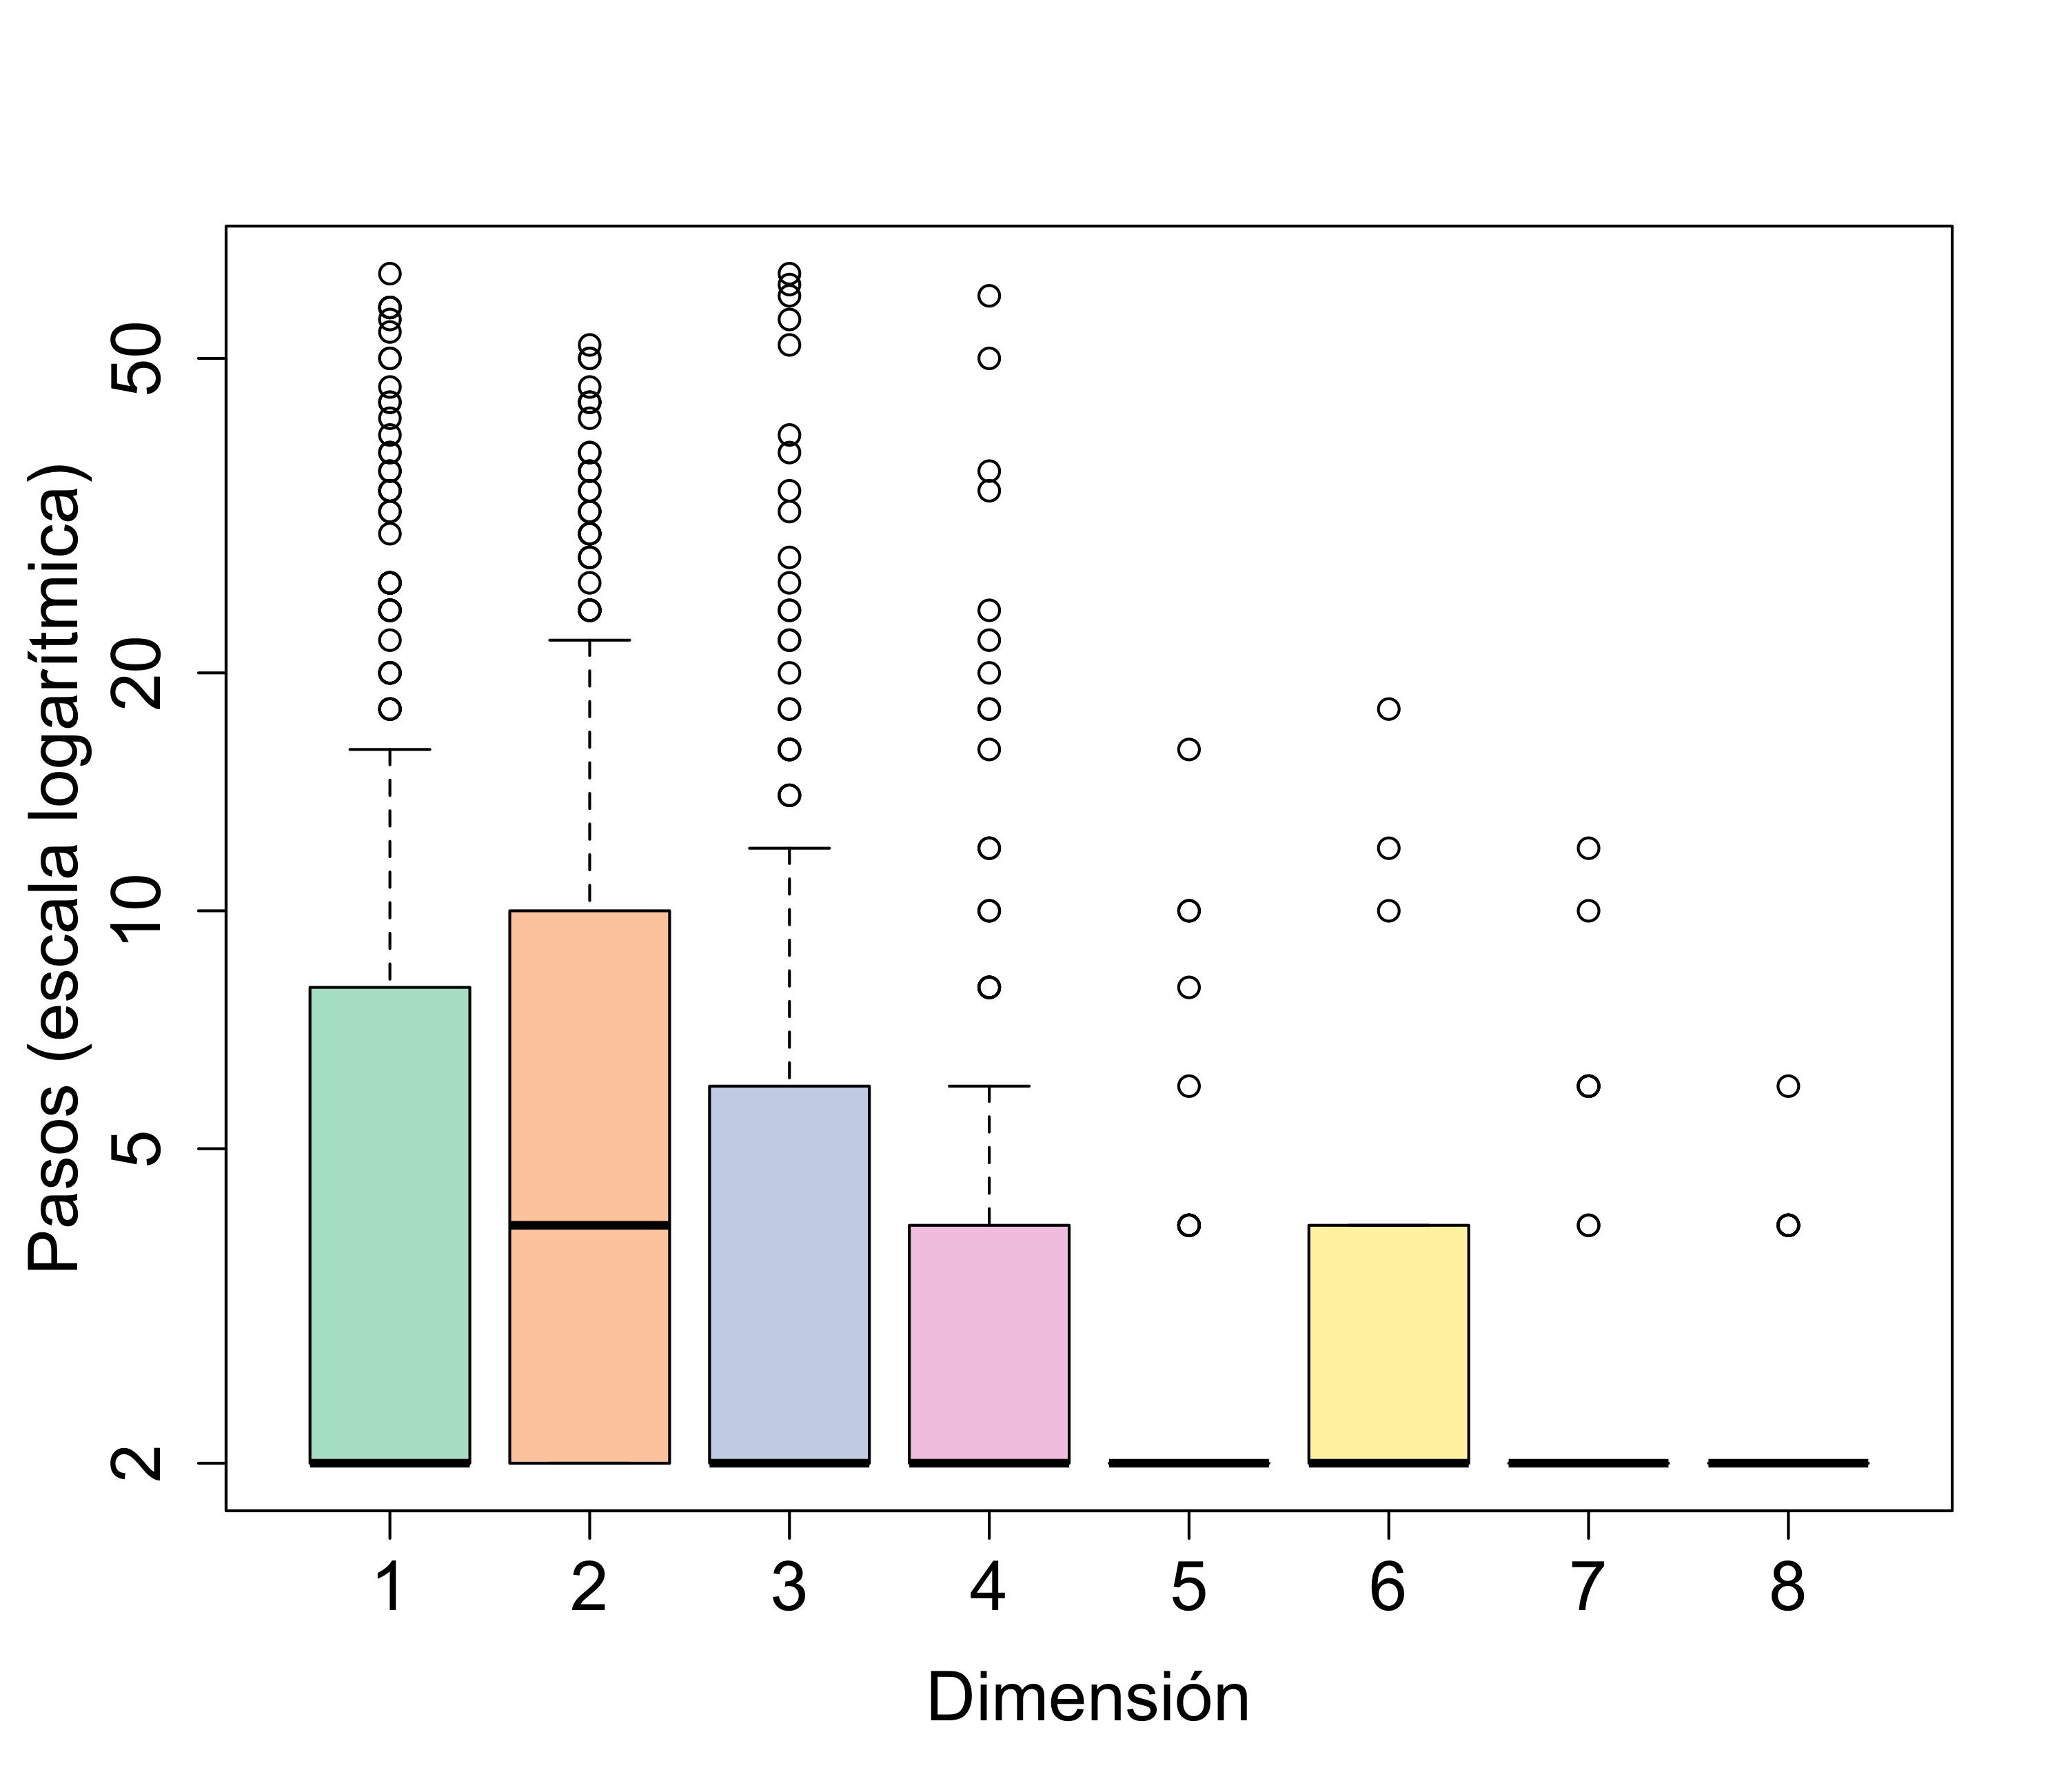
\includegraphics[width=\linewidth]{Largo64-pasos.png}
 		\label{64pasos}
 	\end{subfigure}
 	\begin{subfigure}[b]{0.45\linewidth}
 		\caption{Caminata de 128 pasos.}
 		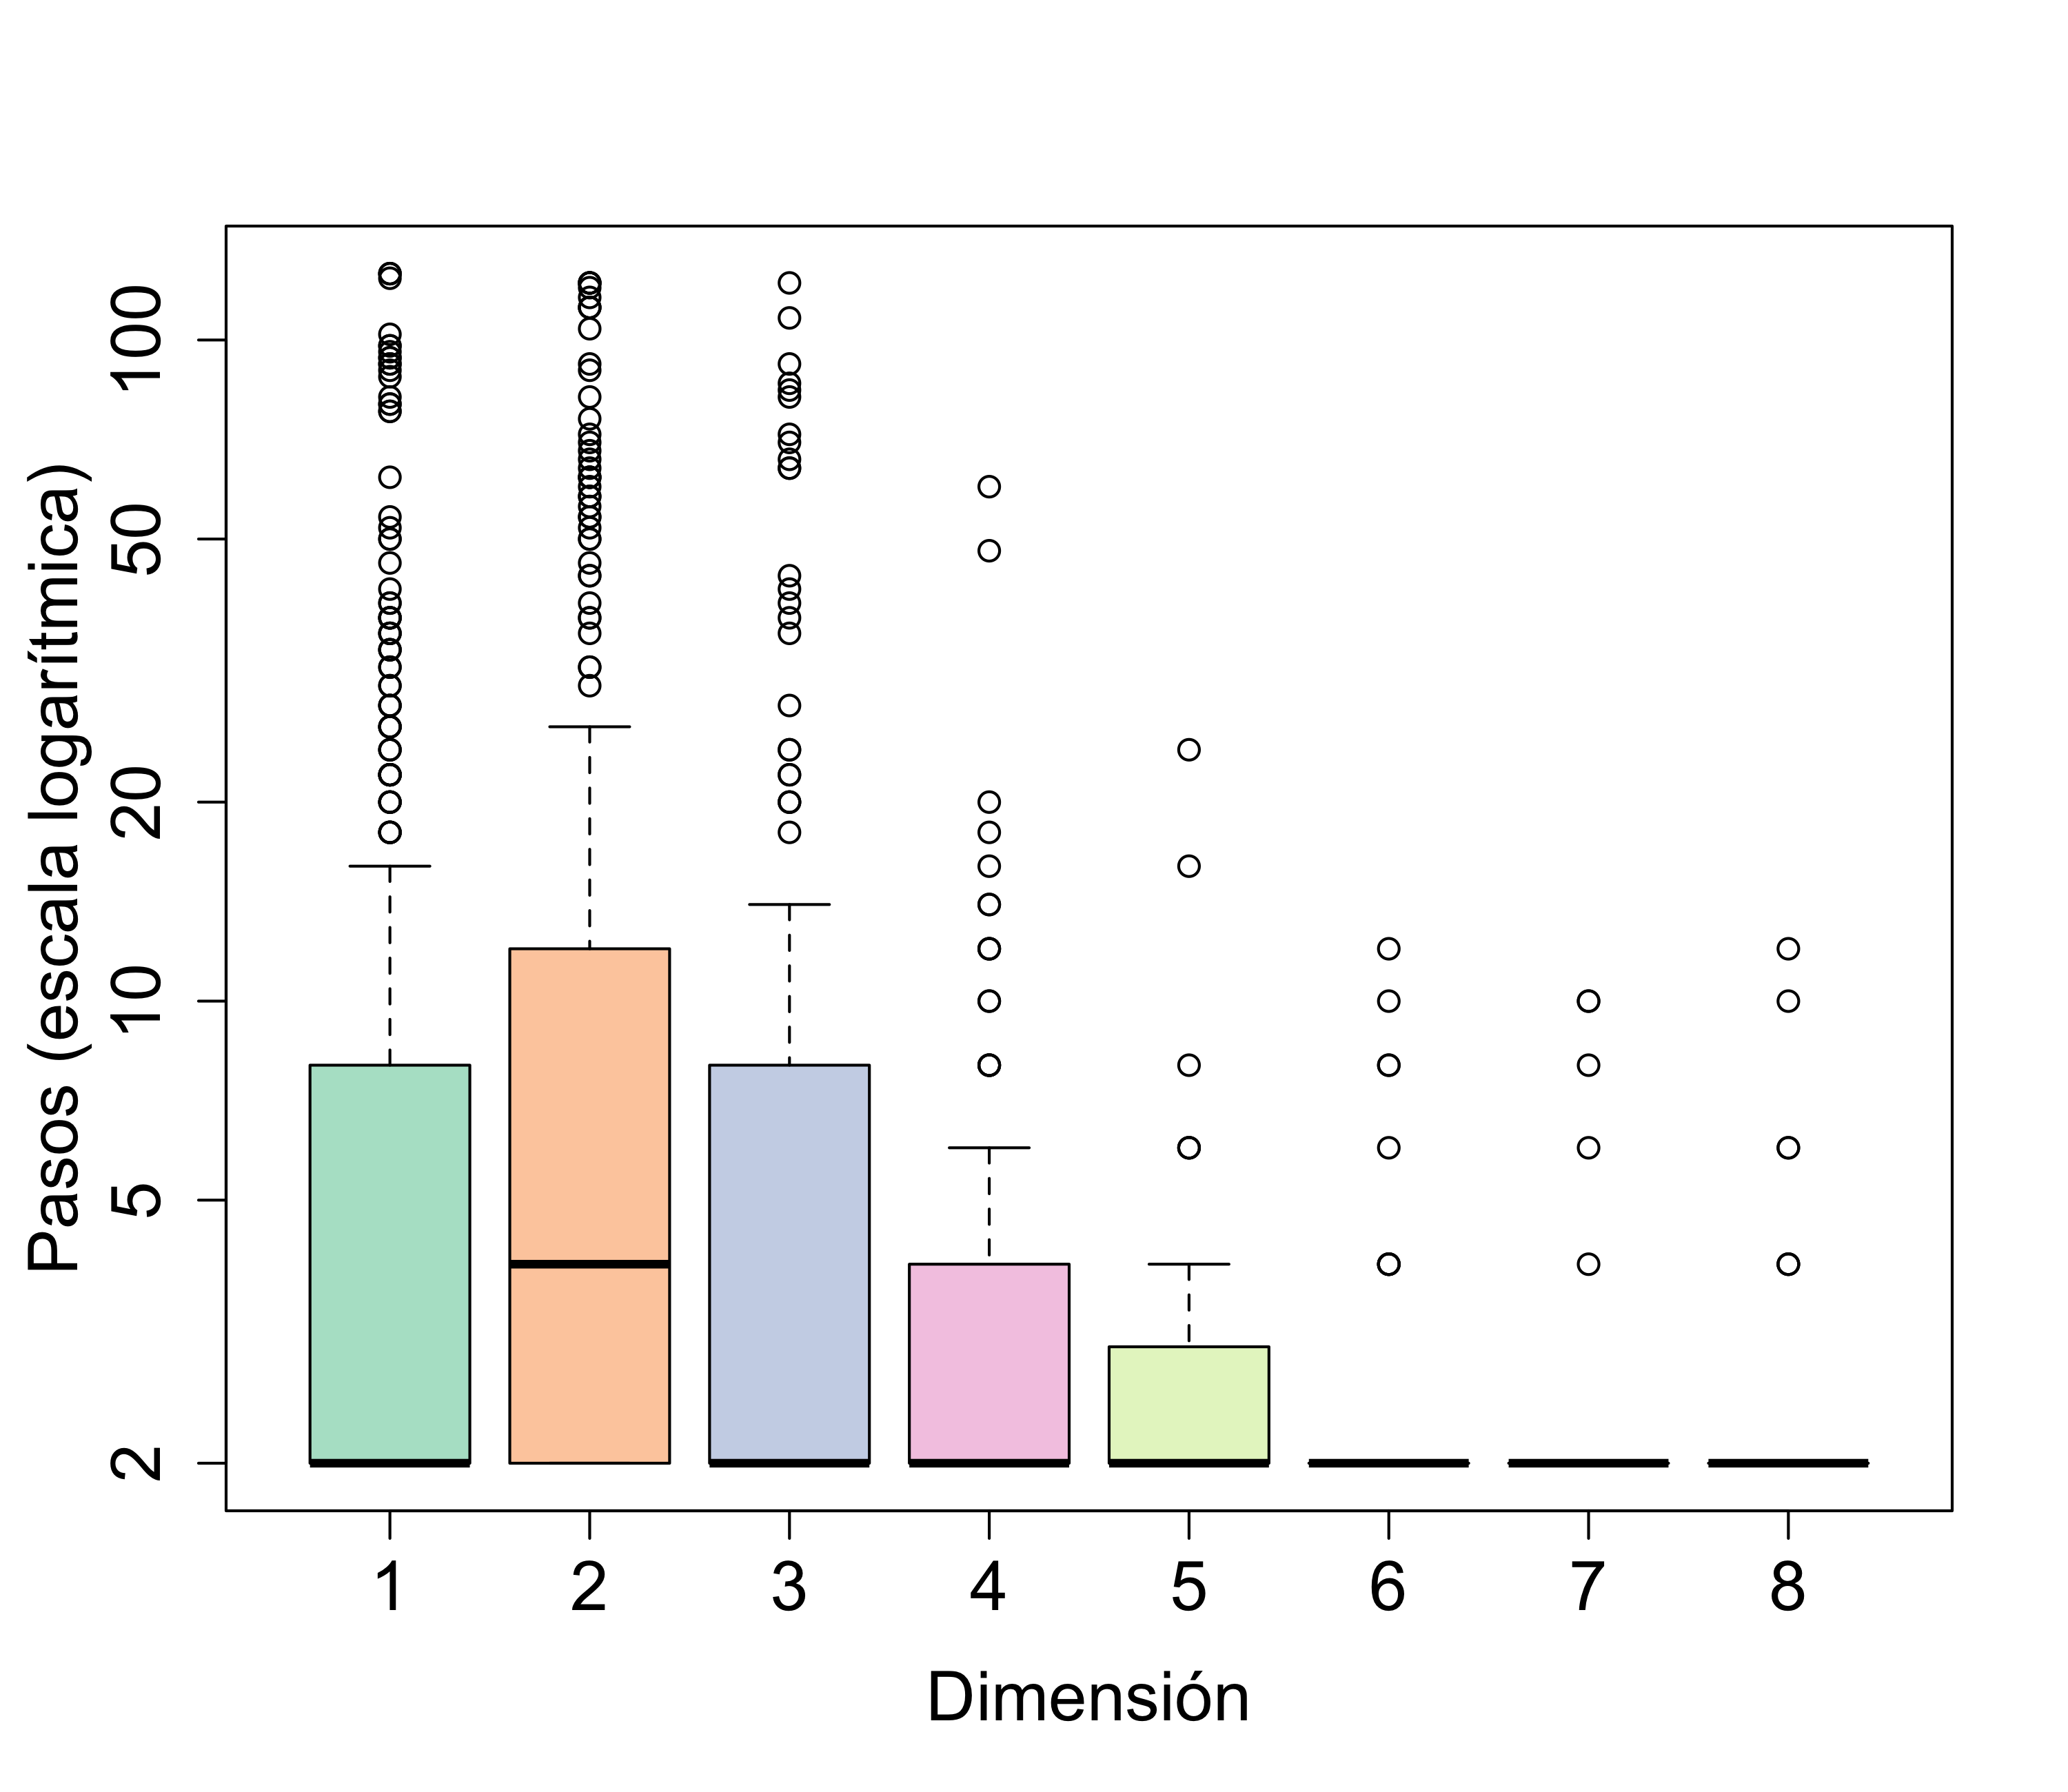
\includegraphics[width=\linewidth]{Largo128-pasos.png}
 		\label{128pasos}
 	\end{subfigure}
	\begin{subfigure}[b]{0.45\linewidth}
 		\caption{Caminata de 256 pasos.}
 		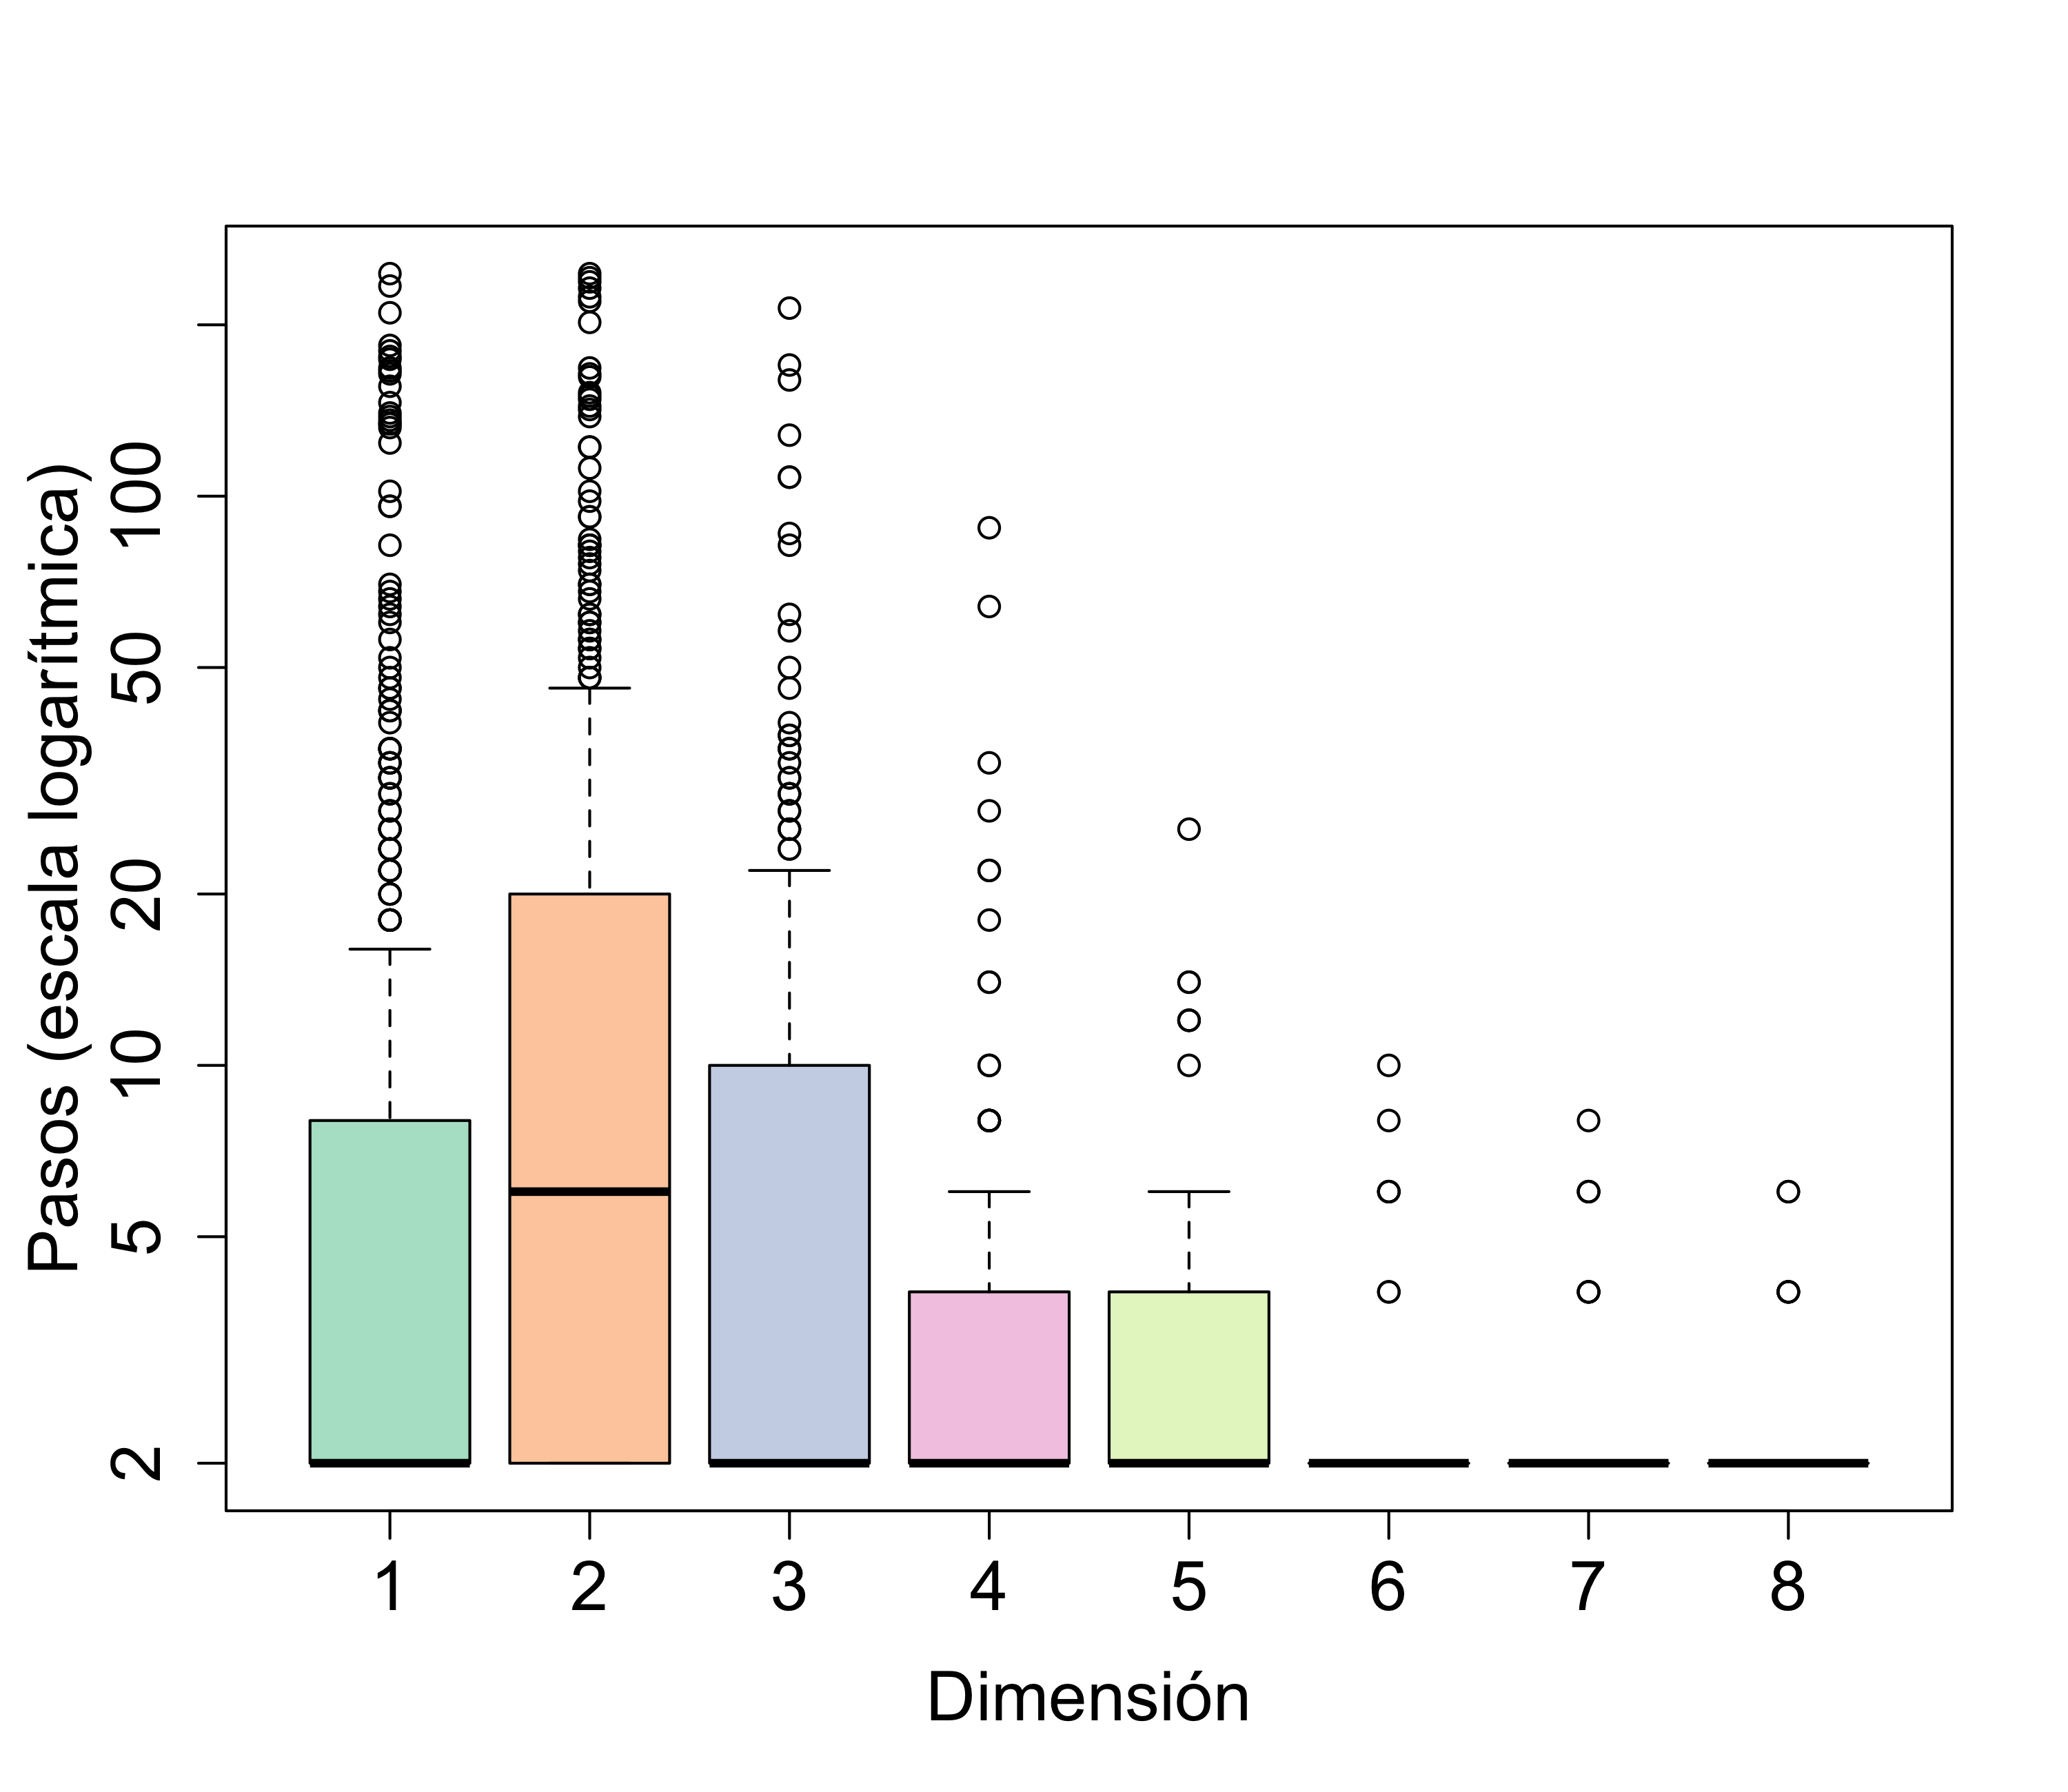
\includegraphics[width=\linewidth]{Largo256-pasos.png}
 		\label{256pasos}
 	\end{subfigure}
 		\begin{subfigure}[b]{0.45\linewidth}
 		\caption{Caminata de 512 pasos.}
 		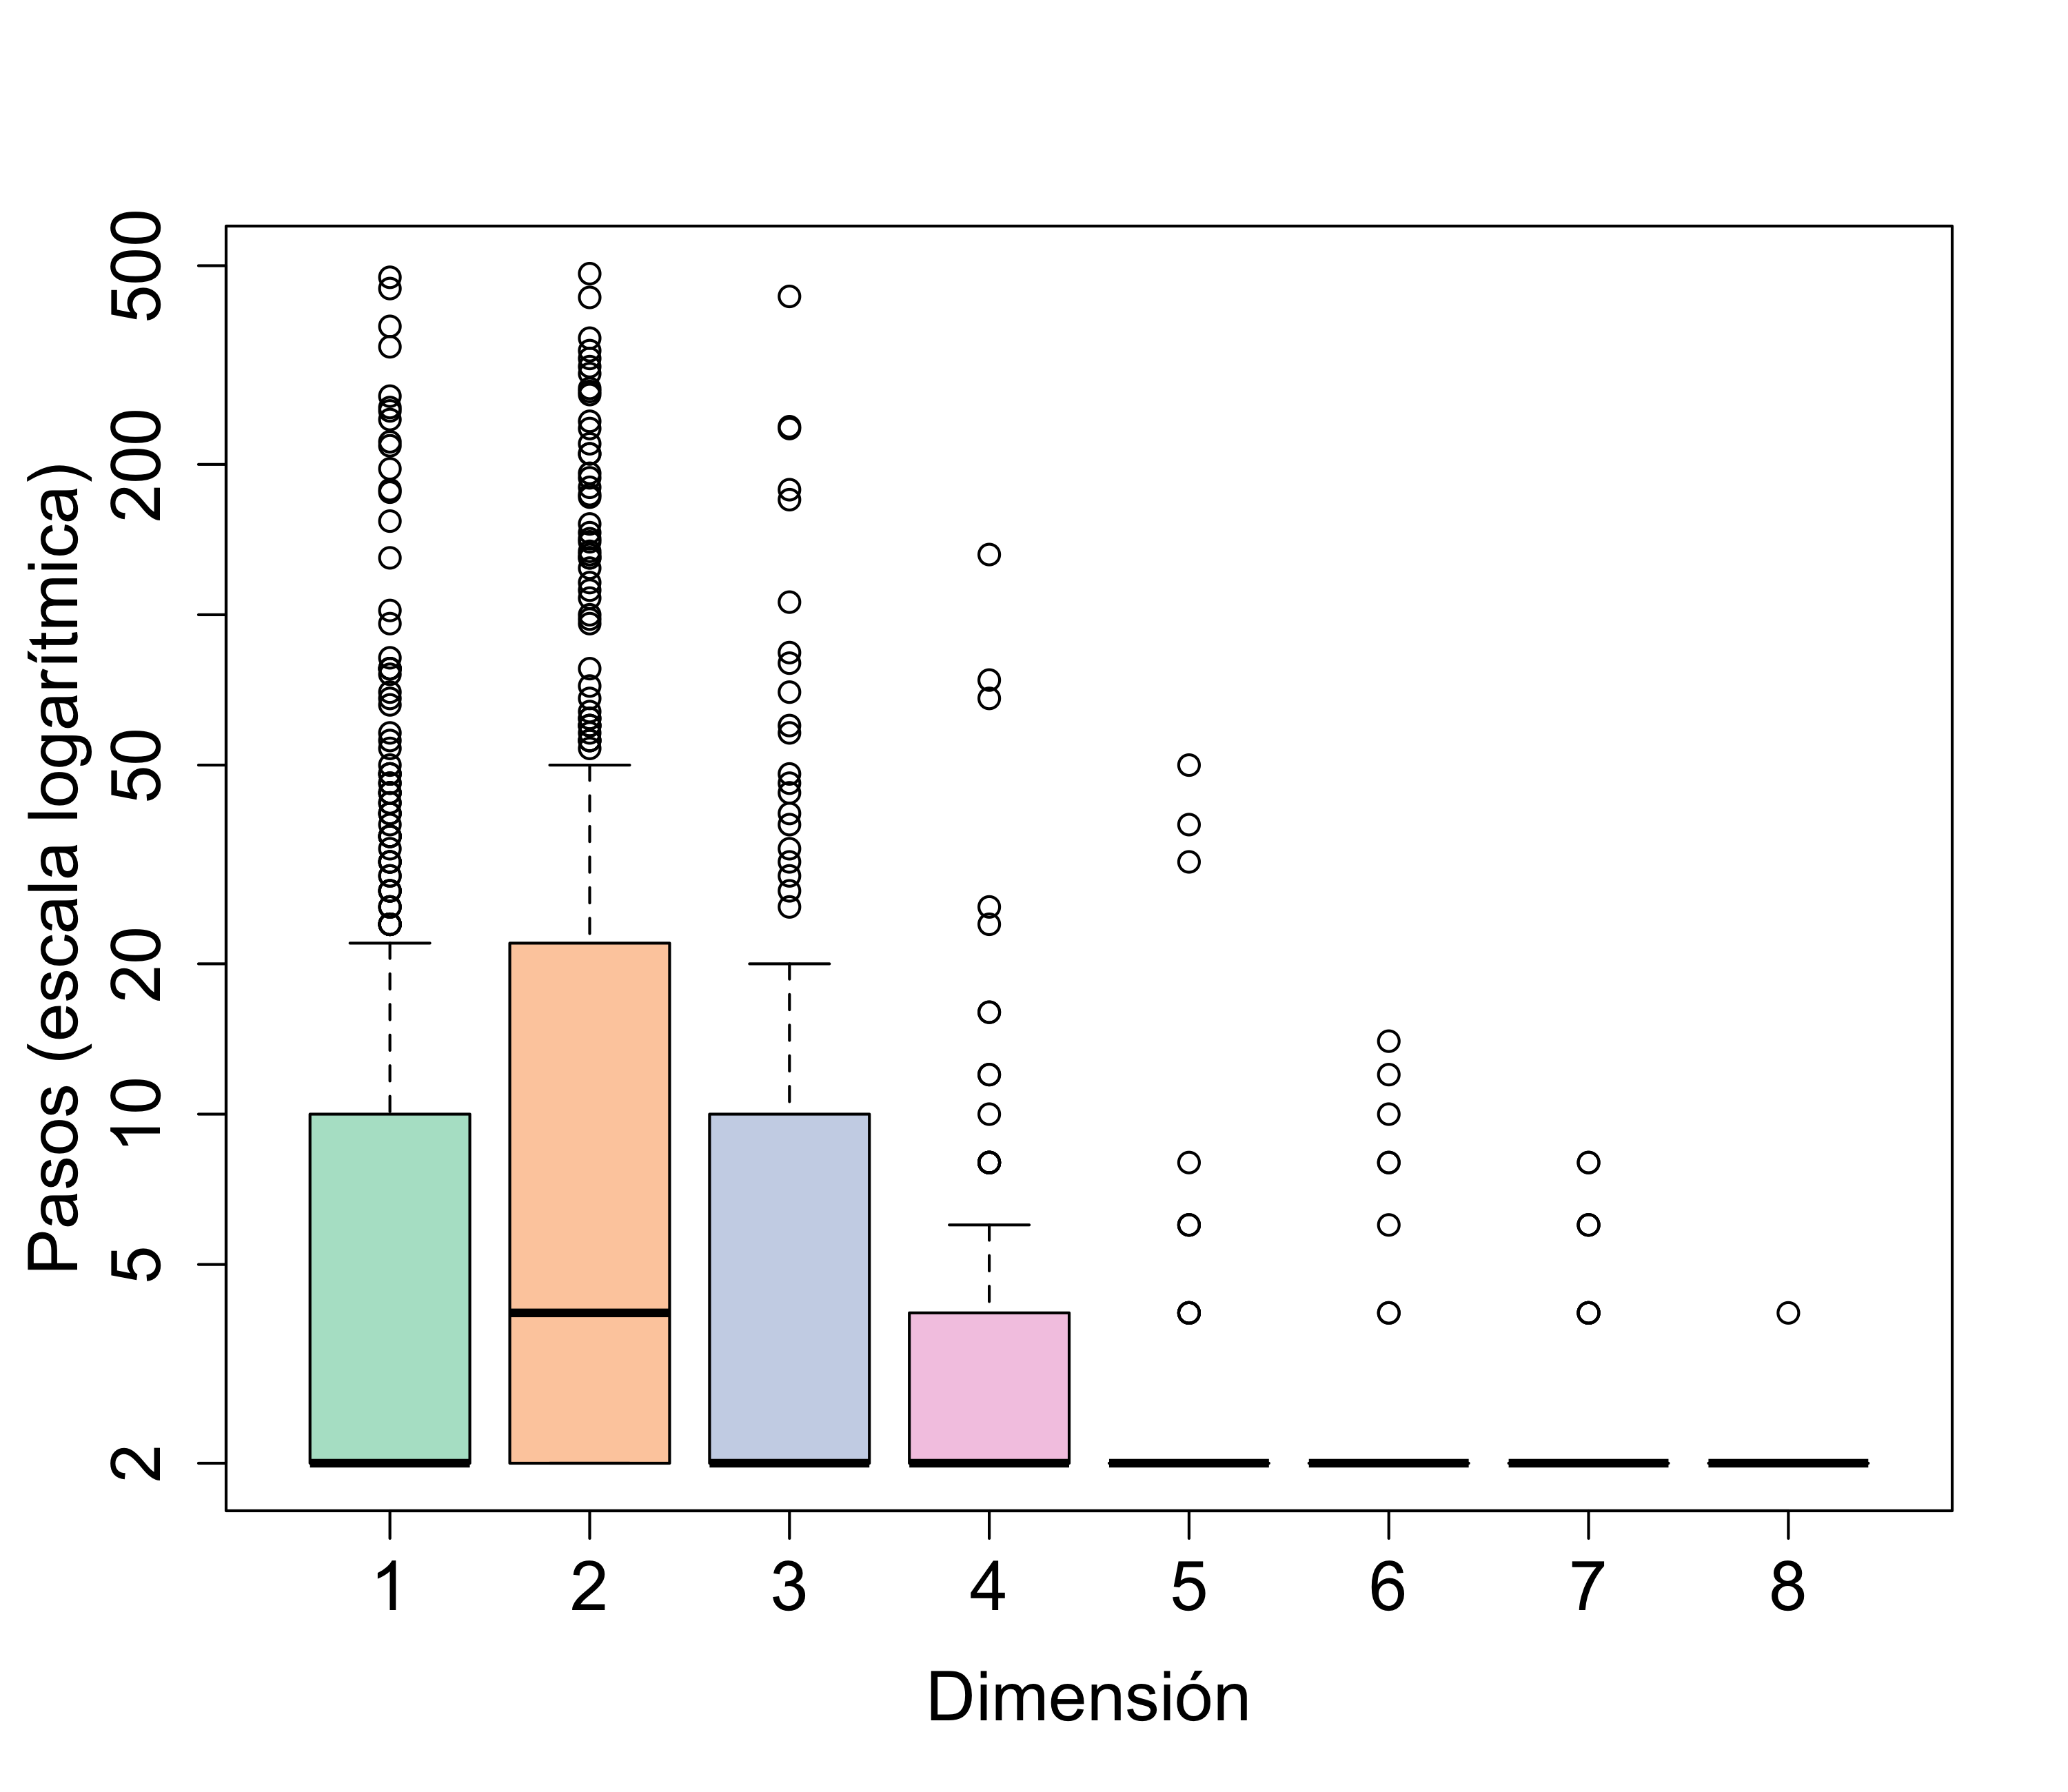
\includegraphics[width=\linewidth]{Largo512-pasos.png}
 		\label{512pasos}
 	\end{subfigure}
 		\begin{subfigure}[b]{0.45\linewidth}
 		\caption{Caminata de 1024 pasos.}
 		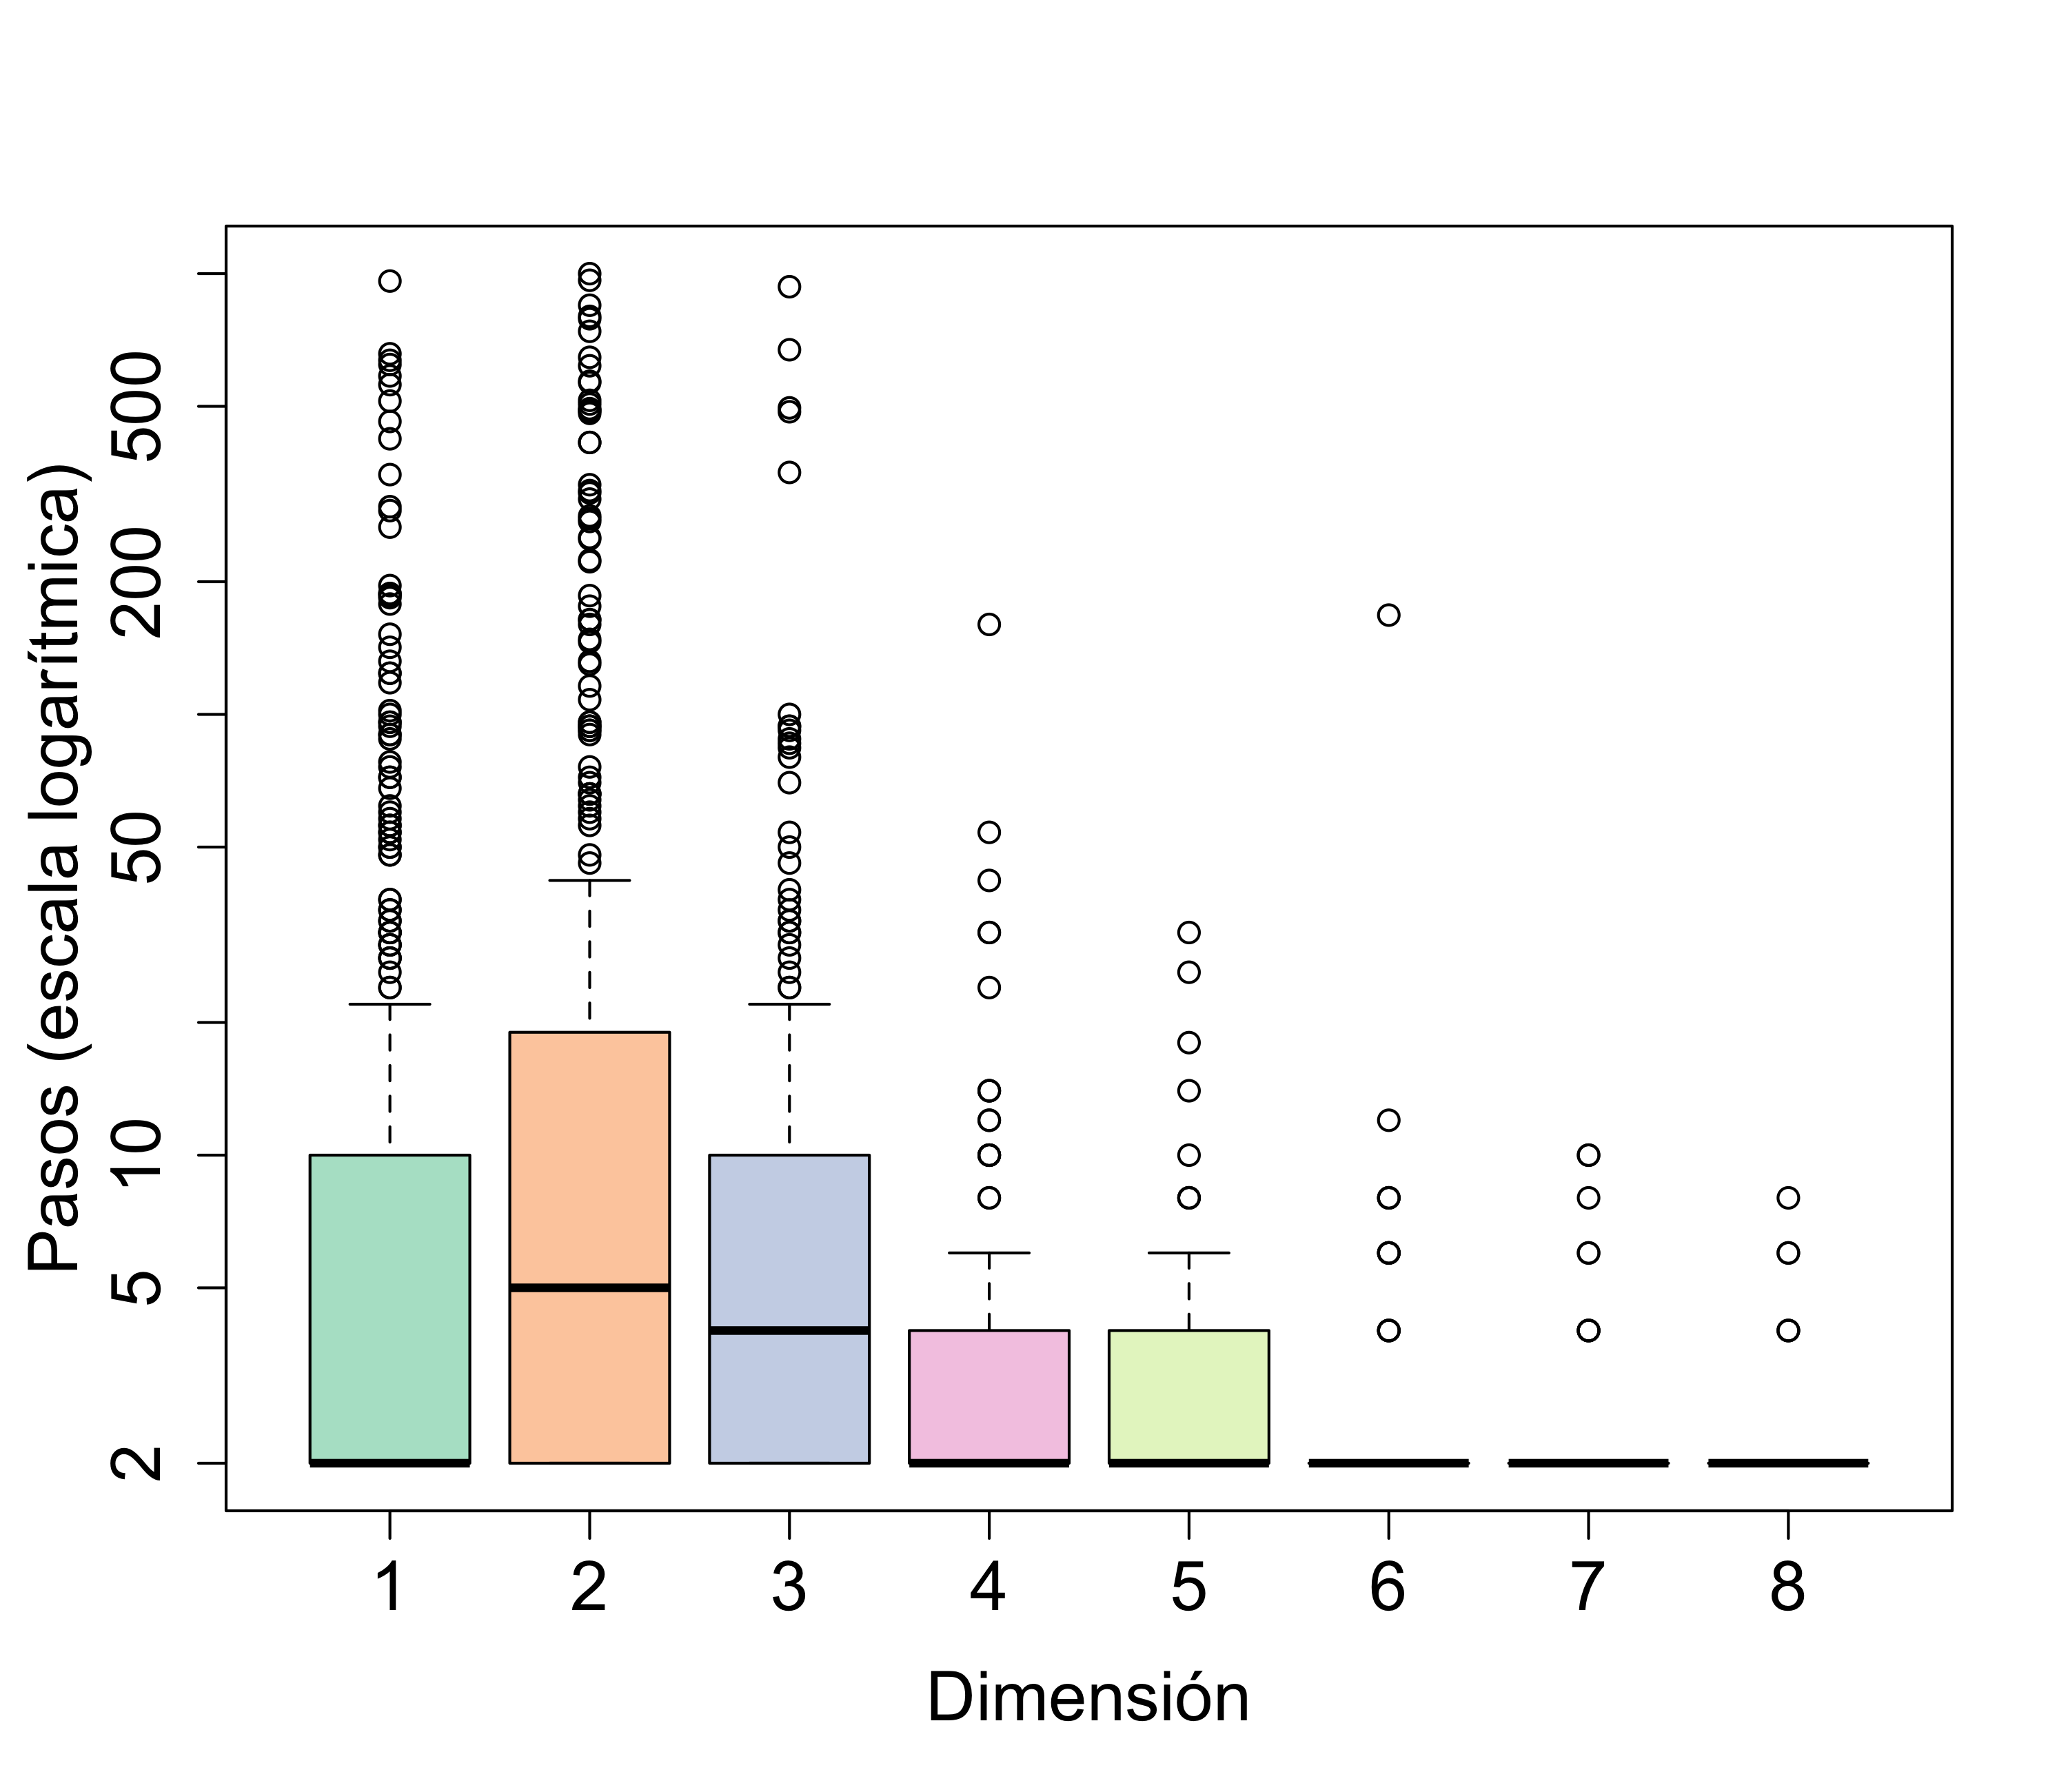
\includegraphics[width=\linewidth]{Largo1024-pasos.png}
 		\label{1024pasos}
 		\end{subfigure}
 		
\label{pasos-log}
 \end{figure}
 

 \bibliographystyle{plain} 
\bibliography{Referencias}
\end{document}